\section{Diseño y resolución}

En este apartado vamos a pasar a explicar los detalles del desarrollo del proyecto. Como se ha dicho, el proyecto consiste en realizar un sistema capaz de seguir los movimientos del balón y las jugadoras de un partido de volleyball mediante imágenes proporcionadas por una cámara en vista cenital.

El seguimiento se puede realizar por \textit{tracking}, sustracción de fondo, o bien un sistema que aúne ambas cosas para una mayor robustez.

Una vez resuelta la parte del seguimiento, el siguiente objetivo sería registrar las posiciones detectadas a un fichero de salida en formato CSV, mediante el cual se puedan hacer análisis de distintas métricas del juego.

El desarrollo se va a centrar, como he ido aclarando, en una aplicación en Python utilizando OpenCV y PyQt para la parte de interfaz gráfica. De cara a la construcción del sistema, la estrategia a seguir es desarrollar separadamente sus partes y posteriormente integrarlas para que funcionen de manera conjunta.

A continuación, detallaré estas partes y cómo se ha resuelto su implementación. Las partes principales del sistema son: sustracción de fondo, seguimiento (\textit{tracking}), interfaz gráfica y métodos de consistencia temporal.

\subsection{Sustracción de fondo}
\label{sec:subtractors}
Para empezar a detectar formas en la imagen, primero nuestro sistema tiene que ser capaz de hacer una estimación del fondo. La técnica mediante la cual se hace esto se denomina sustracción de fondo. Esta es, por tanto, una parte primordial de nuestro sistema que debe funcionar de una manera suficientemente robusta. Este debe ser capaz, además, de distinguir a las jugadoras del balón, y de etiquetar cada una de las formas de una manera consistente entre los frames del vídeo. Para lograr esta serie de objetivos, no bastará con la salida de los sustractores, sino que tendremos que procesarla con una serie de operaciones.

No obstante, primero tendremos que solucionar el problema principal, la sustracción de fondo. Teniendo en cuenta que las imágenes proceden de una cámara fija y cenital, y que por tanto el fondo siempre va a ser exactamente el mismo, una primera aproximación ingenua a este problema podría ser tan simple como realizar una diferencia entre los frames del video, usando como referencia un frame donde se vea solamente el campo sin ninguna jugadora sobre él.

Por desgracia, las condiciones de iluminación no siempre van a ser totalmente iguales, lo cual va a dificultar en gran medida la detección de objetos usando este método. Además, no siempre vamos a tener disponible una imagen limpia del campo en un vídeo para usar como modelo de fondo. Por ello es complicado realizar un modelo del campo para las diferentes condiciones de iluminación a lo largo de un día mediante la simple resta de frames.

Además de la sensibilidad a cambios en la iluminación, este método adolece de otra desventaja: no es capaz de detectar sombras. Las imágenes que usamos son las de un campo de volleyball dentro de un pabellón, y los focos de dentro de este hacen que sea bastante común tener sombras alargadas y notables en las jugadoras.

Una vez hemos podido ver que esta manera de proceder no es todo lo viable que cabría desear, tendremos que empezar a plantearnos otras opciones a nuestra disposición. OpenCV proporciona distintos algoritmos de sustracción de fondo, los cuales podemos aprovechar y comparar para ver cuál es más apropiado en nuestro propósito.

\begin{figure}
    \centering
    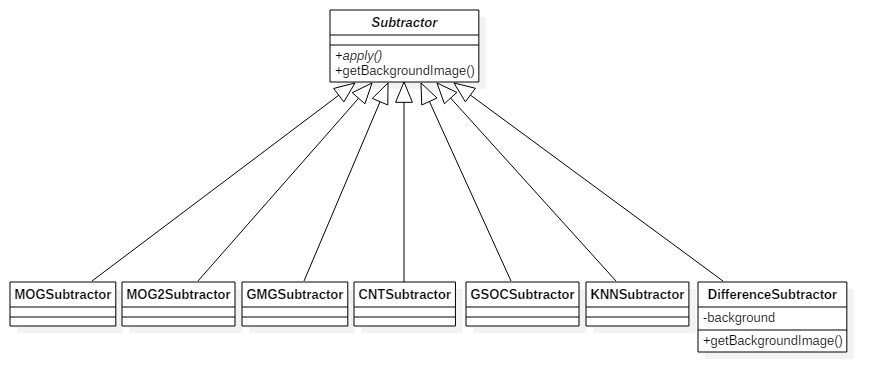
\includegraphics[width=0.9\textwidth]{images/subtractors}
    \caption{Estructura de clases de los sustractores de fondo.}
    \label{fig:subtractors}
\end{figure}

Para facilitar el uso de estos algoritmos, se ha hecho uso de la programación orientada a objetos que nos ofrece Python. Se ha creado una clase abstracta llamada Subtractor de la cual heredan todas las clases que hagan uso de los algoritmos de OpenCV así como el de diferencia de frames. Dicha clase proporciona una interfaz común a todas las clases, que hará más sencillo el uso de ellas. La estructura resultante puede verse en la figura \ref{fig:subtractors}.

El funcionamiento interno de las clases resultantes, como se ha dicho, corresponde a las propias implementaciones de OpenCV. Pasaremos a explicar los fundamentos teóricos de cada uno de estos algoritmos.

\subsubsection*{MOG}
MOG, mezcla de gaussianas (\textit{Mixture of Gaussians}), fue diseñado en 2002 \cite{KaewTraKulPong2002} partiendo de otro algoritmo ya existente de Grimson \textit{et al} \cite{698583,784637,868677}. Usa un modelo de aprendizaje semiparametrizado para estimar el fondo. Ambas versiones crean un modelo del fondo para cada pixel RGB en base a una mezcla de k gaussianas, con $3\leq k \leq 5$, cada una de las cuales representa un color con una cierta variabilidad. La probabilidad de que un pixel tenga el valor $x_N$ en el instante de tiempo $N$ es de
\[
    p(x_N) = \sum_{j=1}^{k} w_j \mathcal{N} (x_N;\theta_j )
\]
donde $w_k$ es el peso de la componente guasiana k-ésima. $\mathcal{N} (x;\theta_k)$ es la ecuación que define la distribución de la componente, representada por
\[
    \mathcal{N}(x;\theta_k) = \mathcal{N}(x;\mu_k, \Sigma_k) = \frac{1}{(2\pi)^{\frac{D}{2}}|\Sigma_k|^\frac{1}{2}}e^{-\frac{1}{2}(x-\mu_k)^T\Sigma_k^{-1}(x-\mu_k)}
\]
donde $\mu_K$ es la media y $\Sigma_K = \sigma_K^2I$ es la matri< de covarianza de la componente. Las distribuciones se ordenan en base a una medida de \textit{fitness}, definido por $\frac{w_k}{\sigma_k}$ y las B primeras forman el modelo de fondo con $B = \arg\min (\sum_{j=1}^{k} w_j < T)$ donde T es el límite de probabilidad mínima a partir de cual un pixel se considera fondo. Un pixel se considera parte de los objetos de la escena si está 2.5 desviaciones por encima de alguna de las B distribuciones.

La diferencia entre la implementación original de Grimson y la de este algoritmo radica simplemente en las funciones de actualización de cada frame. En el caso del original las funciones de actualización son: 
\begin{align*}
    &\hat{w}_k^{N+1} = (1 - \alpha)\hat{w}_k^{N} + \alpha\hat{p}(\omega_k | x_{N+1}) \\
    &\hat{\mu}_k^{N+1} = (1 - \alpha)\hat{\mu}_k^{N} + \rho x_{N+1} \\
    &\hat{\Sigma}_k^{N+1} = (1 - \alpha)\hat{\Sigma}_k^{N} + \rho (x_{N+1} - \hat{\mu}_k^{N+1})(x_{N+1} - \hat{\mu}_k^{N+1})^T \\
    &\rho = \alpha \mathcal{N}(x_{N+1};\hat{\mu}_k^N, \hat{\Sigma}_k^N) \\
    &\hat{p}(\omega_k | x_{N+1}) = \text{1 si $\omega_k$ es la primera componente gaussiana; 0 si no}
\end{align*}

siendo $\alpha$ la velocidad de aprendizaje, o \textit{learning rate} del algoritmo.

Las funciones de actualización de la versión de Kaewtrakulpong añaden ciertas optimizaciones para hacer más robusta la estimación de fondo. Ya que siguen el mismo fundamento que las anteriores, pero son algo más complicadas, no merece la pena explicarlas aquí.

Una novedad de MOG respecto a su predecesor es la capacidad para discernir las sombras de los objetos que las proyectan. El fundamento de ello es emplear una representación cromática de la imagen para reducir la susceptibilidad, aunque también se tiene en cuenta la componente de luminancia. Si un pixel coincide en cromaticidad con la cromaticidad del fondo, y difiere en luminancia por encima de cierto umbral, se marca como sombra.

\begin{figure}
\begin{subfigure}{.5\textwidth}
  \centering
  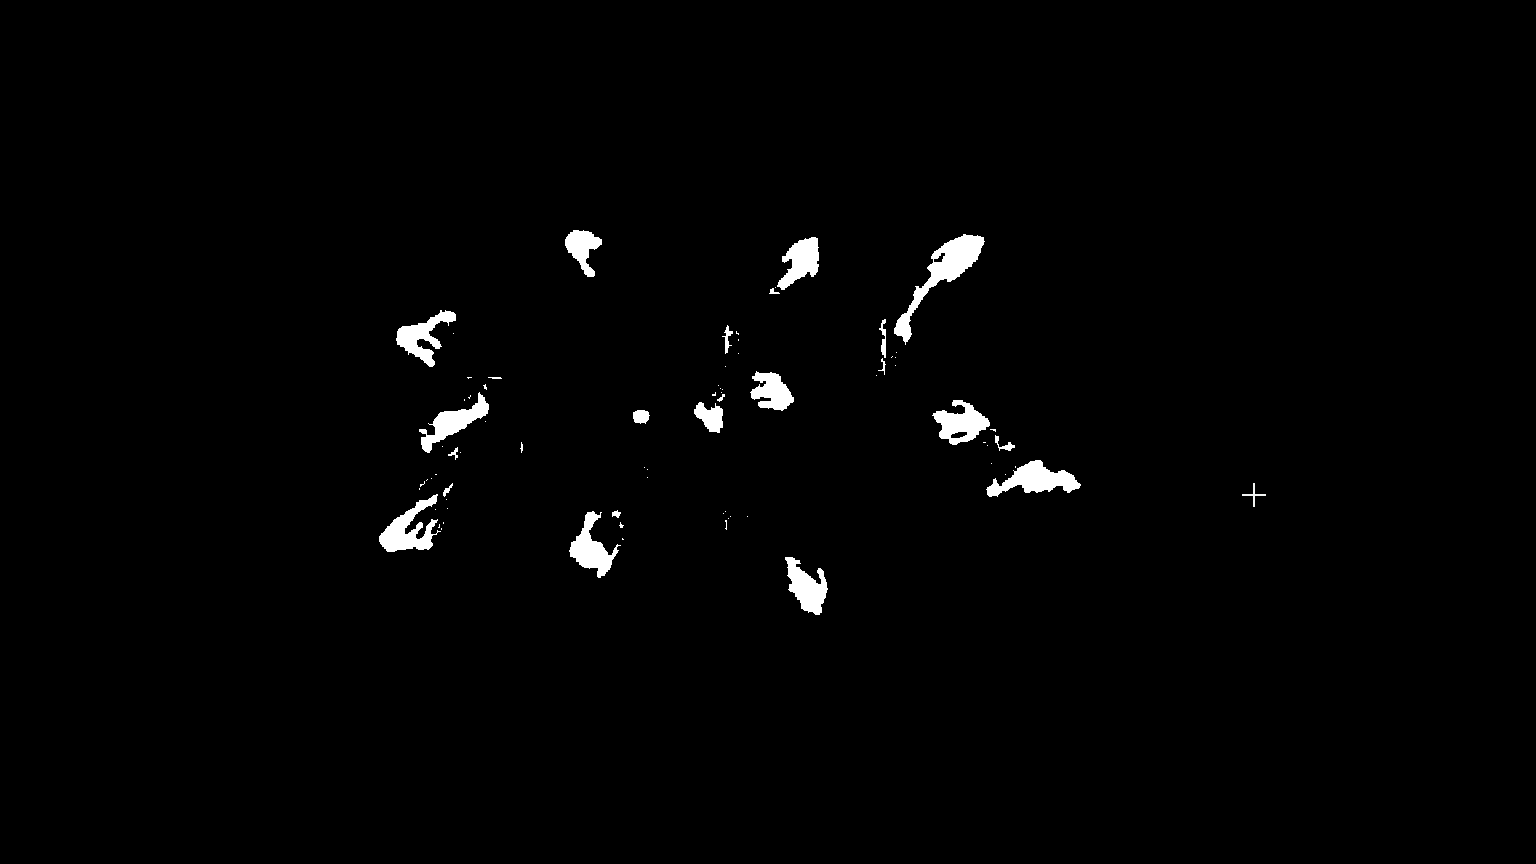
\includegraphics[width=.9\linewidth]{images/MOGsub}
  \caption { }
  \label{fig:MOG1a}
\end{subfigure}%
\begin{subfigure}{.5\textwidth}
  \centering
  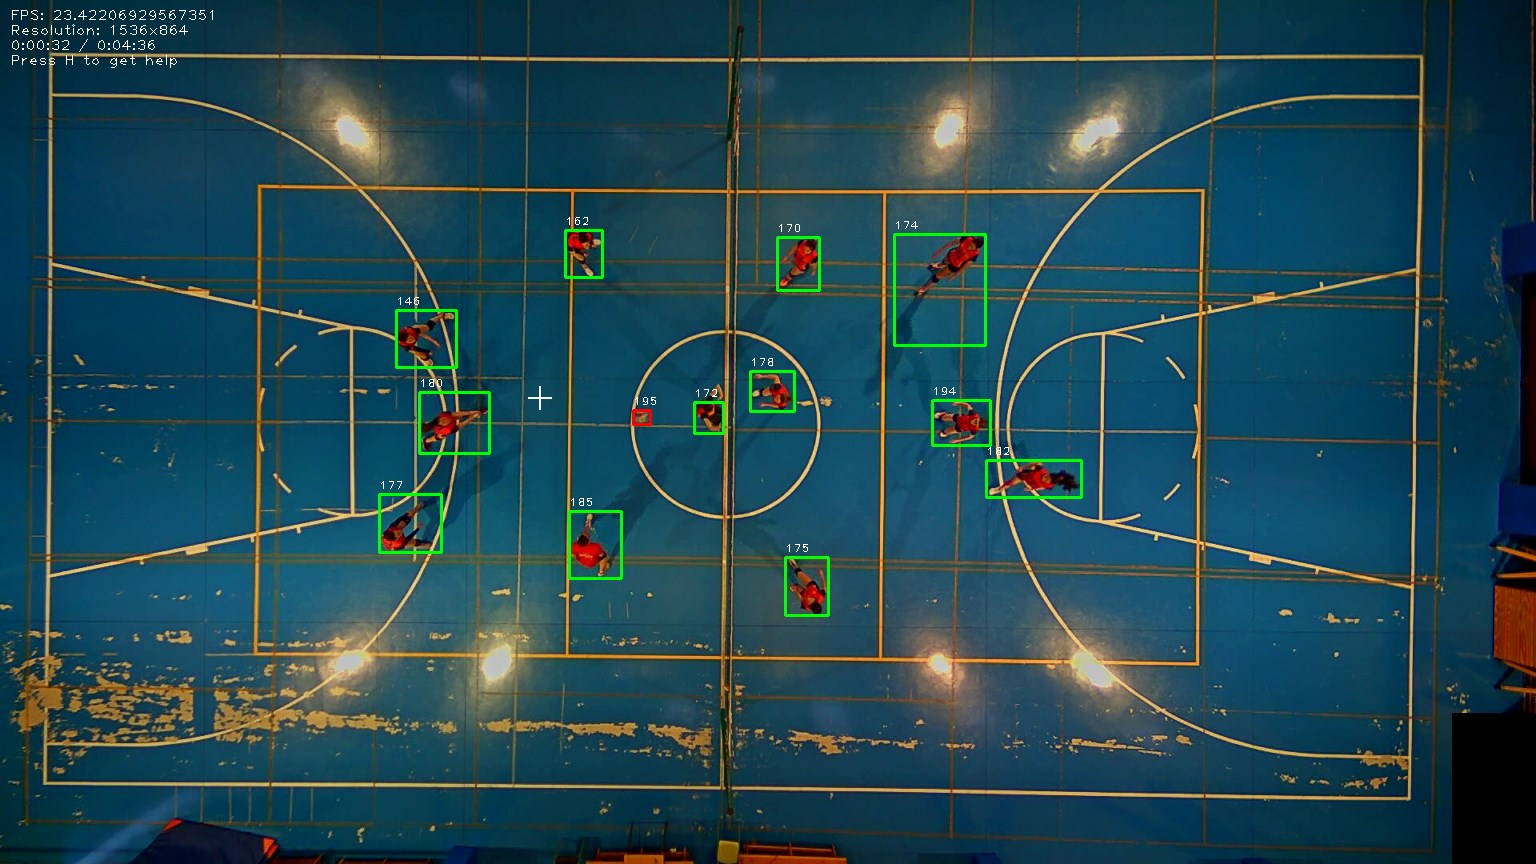
\includegraphics[width=.9\linewidth]{images/MOG}
  \caption { }
  \label{fig:MOG1b}
\end{subfigure}
\caption{Salida del algoritmo MOG: (a) Imagen binarizada del algoritmo. (b) Imagen del vídeo tras aplicar la máscara.}
\label{fig:MOG}
\end{figure}

El funcionamiento de MOG en un frame puede verse en la figura \ref{fig:MOG}. Como puede verse, el algoritmo detecta los cuerpos con cierto nivel de fidelidad, aunque en algunos momentos puede ser especialmente sensible a una jugadora estática. Por otro lado, la detección de las sombras no es en absoluto perfecta, y no en pocas ocasiones se marcan partes de la sombra como componentes de la imagen. El rendimiento es correcto, no se aprecian ralentizaciones graves, como ya comprobaremos más adelante en la tabla \ref{fig:fps}.

\subsubsection*{MOG2}
MOG2 es un algoritmo propuesto en los trabajos \cite{art:Zivkovic1} y \cite{art:Zivkovic2} de Z. Zivkovic. Tiene el mismo fundamento que el anterior método, estima el fondo mediante K gaussianas, haciendo uso nuevamente de un modelo semiparametrizado. 

La diferencia respecto a MOG es que, en lugar de mantener la distribución de mezcla de K gaussianas para todos los pixeles de la imagen, este método es capaz de adaptarse automáticamente y seleccionar el número de componentes gaussianas necesario para cada pixel. Esto permite una mayor flexibilidad e incluso mayor eficiencia, ya que en el peor de los casos podría tener pixeles con el mismo número de componentes que usaría el anterior, pero otros con menos, agilizando la computación.

\begin{figure}
\begin{subfigure}{.5\textwidth}
  \centering
  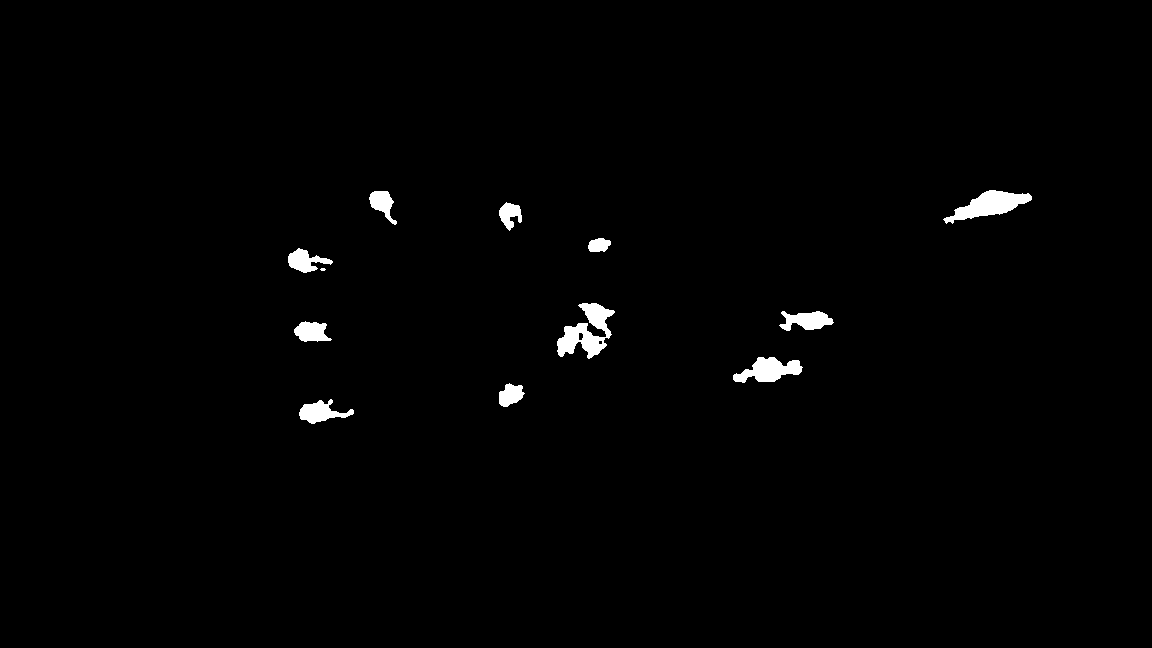
\includegraphics[width=.9\linewidth]{images/MOG2sub}
  \caption { }
  \label{fig:MOG21a}
\end{subfigure}%
\begin{subfigure}{.5\textwidth}
  \centering
  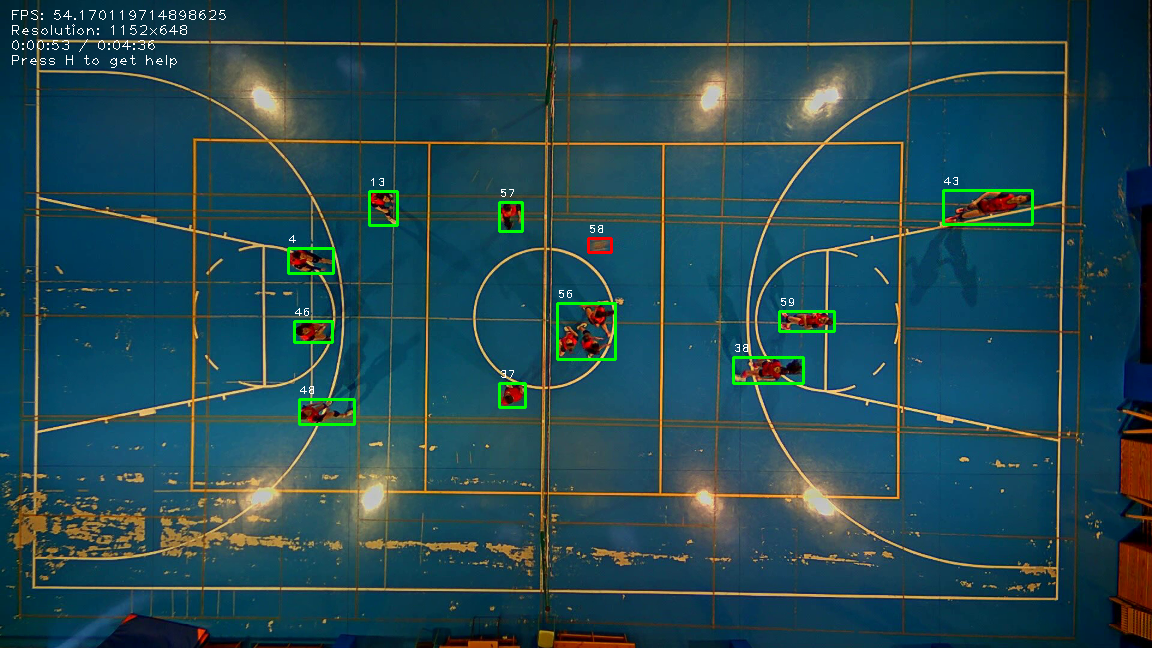
\includegraphics[width=.9\linewidth]{images/MOG2}
  \caption { }
  \label{fig:MOG21b}
\end{subfigure}
\caption{Salida del algoritmo MOG2: (a) Imagen binarizada del algoritmo. (b) Imagen del vídeo tras aplicar la máscara.}
\label{fig:MOG2}
\end{figure}

\subsubsection*{GMG}
GMG surge en un trabajo de Godbehere \textit{et al.} \cite{art:Godbehere}. En este trabajo aclaran los autores que se inspiraron en los algoritmos ya existentes en OpenCV. A diferencia de MOG y MOG2, que emplean modelos de distribuciones gaussianas para estimar el fondo de la imagen, GMG emplea un histograma. Por tanto, es un modelo no paramétrico.

La implementación de OpenCV tiene una peculiaridad respecto al resto, y es que requiere de un número $T$ de frames determinado para inicializar el modelo de fondo, y durante estos T frames, la salida del sustractor es una imagen negra. Esta inicialización puede ser interesante en caso de contar con vídeos en los que se vea el fondo al principio sin ningún tipo de oclusión, en nuestro caso, que se vea el campo sin ningún jugador. Desgraciadamente, esto no siempre es posible, por lo que la efectividad inicial puede verse limitada debido a esta condición.

Durante la inicialización, se guarda un histograma $\hat{H}_{ij}(k)$ en el espacio RGB por cada pixel previamente cuantizado. Los primeros $T$ frames del vídeo se utilizan como datos de entrenamiento para estimar la función de probabilidad de cada pixel, es decir, el modelo de fondo. El proceso de inicialización comienza en cada frame generando un vector $f_{ij}(k) = L(\hat{I}_{ij}(k)) \in \mathcal{F}$ mediante una función $L$ a partir de la entrada. Una vez generados todos los vectores, se calcula el histograma $\hat{H}_{ij}(T) = \frac{1}{F_{tot}}\Sigma_{x = 1}^T f_{ij}(x)$. $F_{tot}$ es el número total de distintas características (\textit{features}) observadas, que siempre debe ser menor o igual que $F_{max}$, una constante del sistema. En caso de que sea mayor, se eliminan las observaciones más antiguas hasta que se cumpla que $F_{tot} \leq F_{max}$.

A partir de aquí se utiliza inferencia bayesiana para calcular la probabilidad de que un pixel dado sea fondo a partir de la característica observada. Sea $p(F|f)$ la probabilidad de que un pixel con característica $f_{ij}(k)$ sea parte del primer plano y $p(B|f)$ la probabilidad de que este mismo pixel sea fondo:
\[
    p(B|f) = \frac{p(f|B)p(B)}{p(f|B)p(B)+p(f|F)p(F)}
\]

Siendo $p(f|B) = f_{ij}(k)^T\hat{H}_{ij}(k)$, $p(f|F) = 1 - p(f|B)$, $p(F)$ un parámetro constante que afecta a la sensibilidad del algoritmo y $p(B) = 1 - p(F)$. Una vez calculado $p(B|f)$ para cada pixel, obtenemos una imagen $P(k)$ a la que se le aplican una serie de transformaciones morfológicas de manera que se eliminen las posibles pequeñas formas anómalas que puedan detectarse y las componentes de la imagen aparezcan conectadas. Posteriormente, se aplica un umbral a la imagen para generar a partir de ella una imagen en binario que servirá como máscara y será la salida del sustractor.

Por último, se debe actualizar el histograma que se usa como modelo de fondo de manera que se adapte a posibles cambios en la escena. Si un pixel está marcado como frente de la escena, el histograma para él no se actualiza. Si no, si la característica $f_{ij}(k)$ tiene peso 0 en el histograma y se ha excedido la constante $F_max$, se debe eliminar alguna característica del histograma, la de menor peso. A continuación se actualiza el histograma con la nueva característica a añadir: $H_{ij}(k+1)=(1-\alpha)H_{ij}(k)+\alpha f_{ij}(k)$ siendo $\alpha$ el parámetro de adaptación (\textit{learning rate}) del algoritmo, y cuanto más grande sea, antes se eliminan las observaciones anteriores.

\begin{figure}
\begin{subfigure}{.5\textwidth}
  \centering
  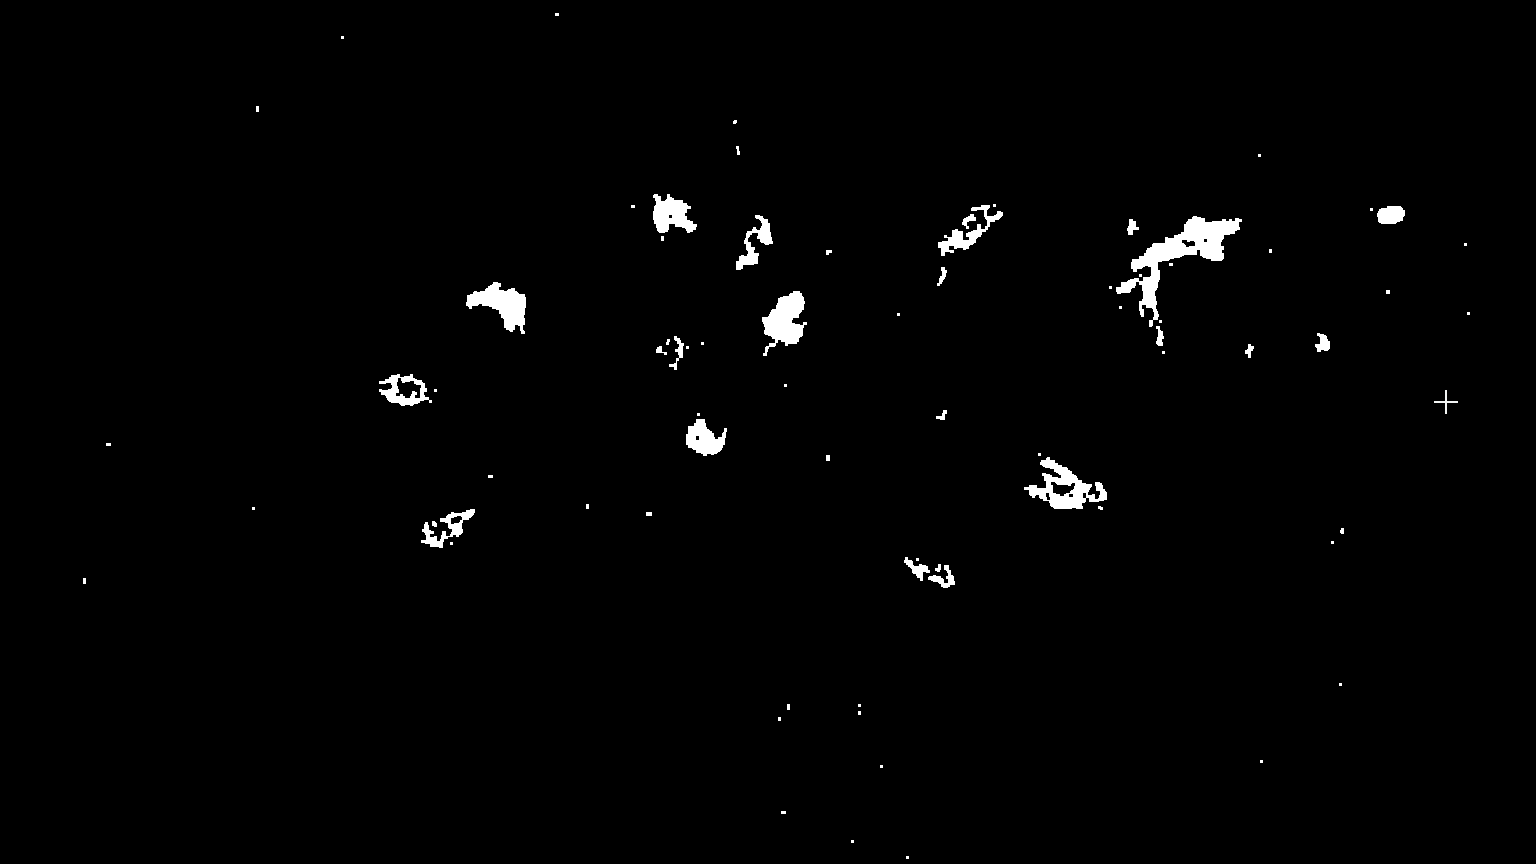
\includegraphics[width=.9\linewidth]{images/GMGsub}
  \caption { }
  \label{fig:GMG1a}
\end{subfigure}%
\begin{subfigure}{.5\textwidth}
  \centering
  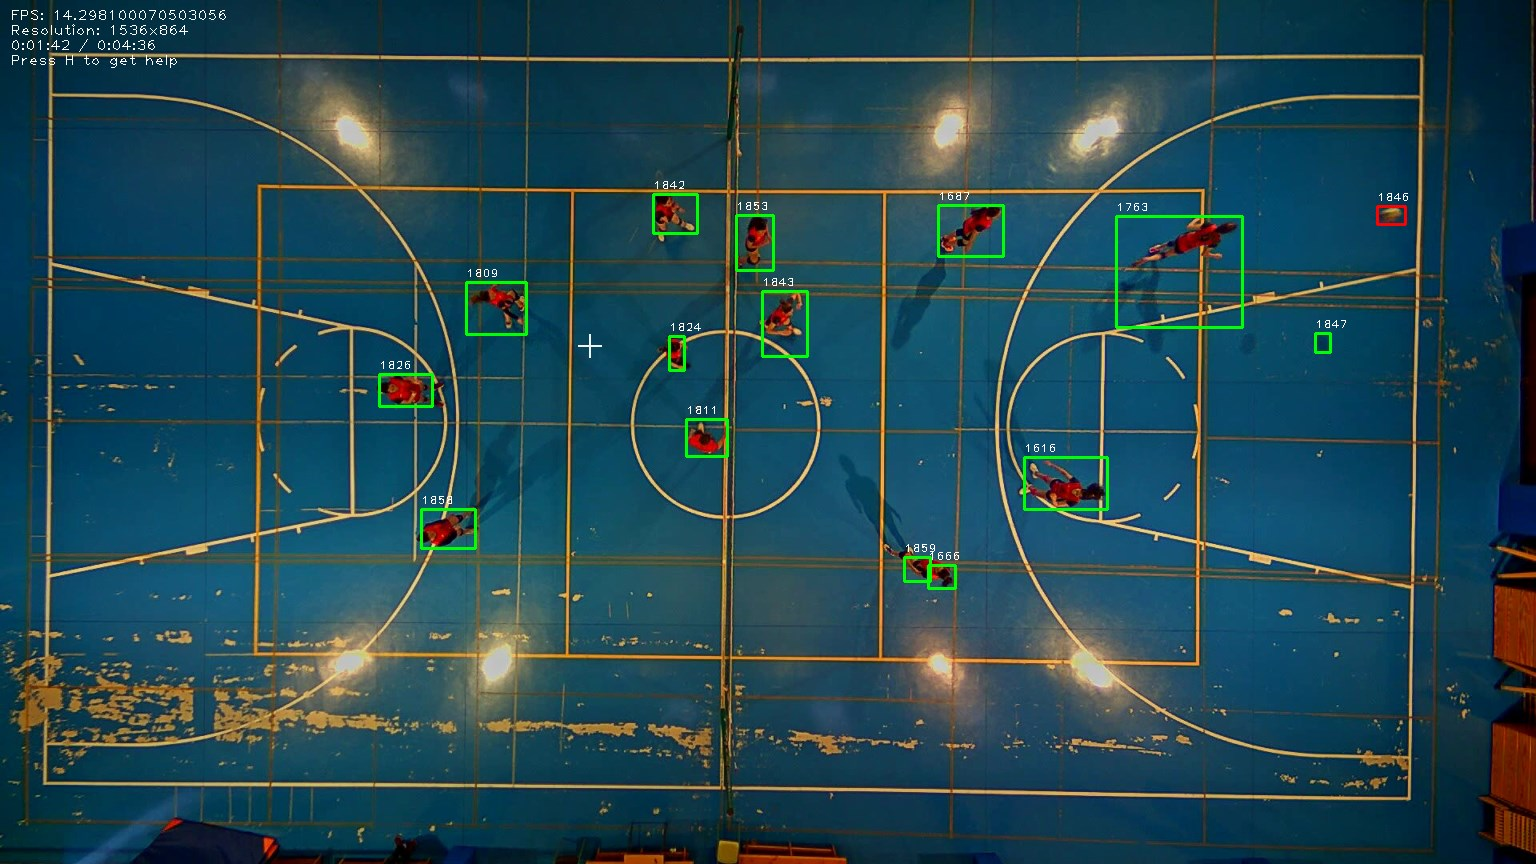
\includegraphics[width=.9\linewidth]{images/GMG}
  \caption { }
  \label{fig:GMG1b}
\end{subfigure}
\caption{Salida del algoritmo GMG: (a) Imagen binarizada del algoritmo. (b) Imagen del vídeo tras aplicar la máscara.}
\label{fig:GMG}
\end{figure}

En cuanto al desempeño del algoritmo, en la figura \ref{fig:GMG} podemos ver que es extremadamente sensible al ruido de la cámara, cosa que hace que la detección de objetos no sea todo lo estable que cabría desear. Esta inestabilidad hace que constantemente se pierdan de un frame a otro algunos de los contornos, y haya que asignarles etiquetas nuevas, lo que explica que en la imagen haya etiquetas tan altas (hablaremos sobre ellas con más profundidad en secciones posteriores). Se aprecian algunos fallos en la detección de sombras, por ejemplo, los de la jugadora más arriba a la derecha y el balón en la imagen. 

El rendimiento no es especialmente bueno, se puede apreciar que cuando el ruido de imagen es muy grande y se detectan muchos contornos falsos, el funcionamiento es extremadamente lento. Además, durante los frames de inicialización, también se notan algunos bajones de FPS (que veremos en la tabla \ref{fig:fps}). Con todo, estos problemas no son especialmente serios y un reescalado de la imagen bastaría para paliarlos.


\subsubsection*{CNT}
Este método fue desarrollado como open source en \cite{git:CNT}. El algoritmo fue planteado por el desarrollador para que fuera eficiente en máquinas de bajo rendimiento, como Raspberry Pi. Se basa en una simple heurística de ``contar'' (que es de donde viene su nombre) cuántos frames se mantiene estable un pixel, y a mayor estabilidad, mayor probabilidad de que este sea fondo.

El método consta de 2 parámetros principales: \textit{minPixelStability} y \textit{maxPixelStability}. La utilidad de estos parámetros es, respectivamente, indicar el número de frames que un pixel debe mantenerse en el mismo color para ser considerado estable, y el máximo crédito que se le permite a un pixel en el histograma.

El algoritmo es relativamente sencillo en su funcionamiento: en cada frame se calcula la diferencia entre el color actual y el del frame anterior, si no se diferencian por encima de cierto límite, se incrementa la estabilidad del pixel en cuestión. Cuando la estabilidad de un pixel llega a ser igual o mayor que la que se le pasa al algoritmo por parámetro se empieza a considerar parte del fondo.

Existe la opción de añadir el uso de un histograma, y aquí es donde cobra importancia el segundo parámetro. Además de llevar un conteo de la estabilidad del propio pixel, se mantiene un histograma con las estabilidades que ha tomado este, y si un pixel supera el valor máximo se deja de sumar. De esta manera el algoritmo puede reponerse rápidamente a que un objeto que ha pasado largo tiempo en escena se mueva.

\begin{figure}
\begin{subfigure}{.5\textwidth}
  \centering
  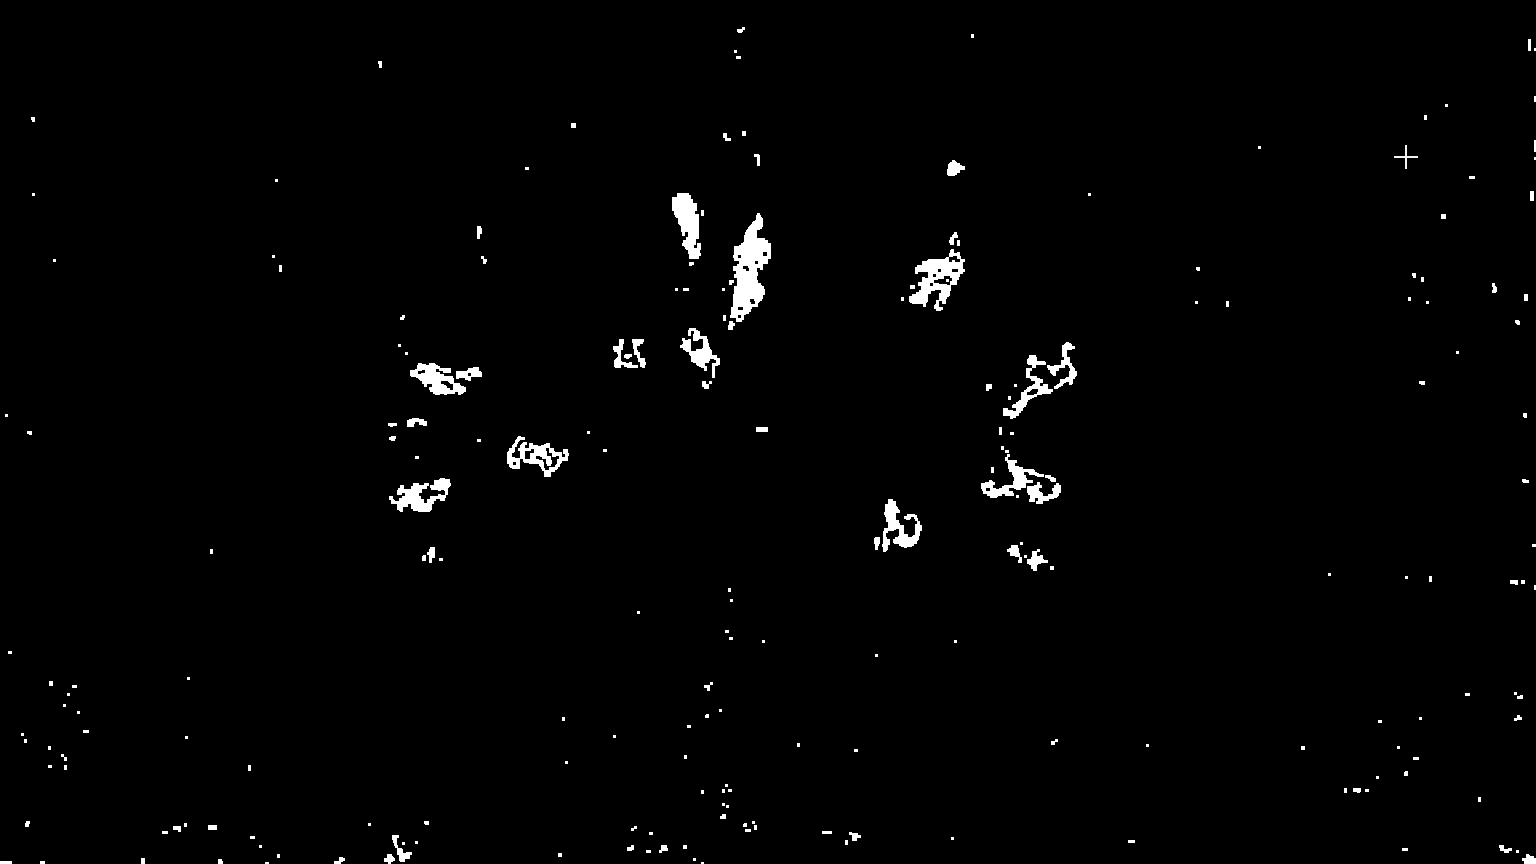
\includegraphics[width=.9\linewidth]{images/CNTsub}
  \caption { }
  \label{fig:CNT1a}
\end{subfigure}%
\begin{subfigure}{.5\textwidth}
  \centering
  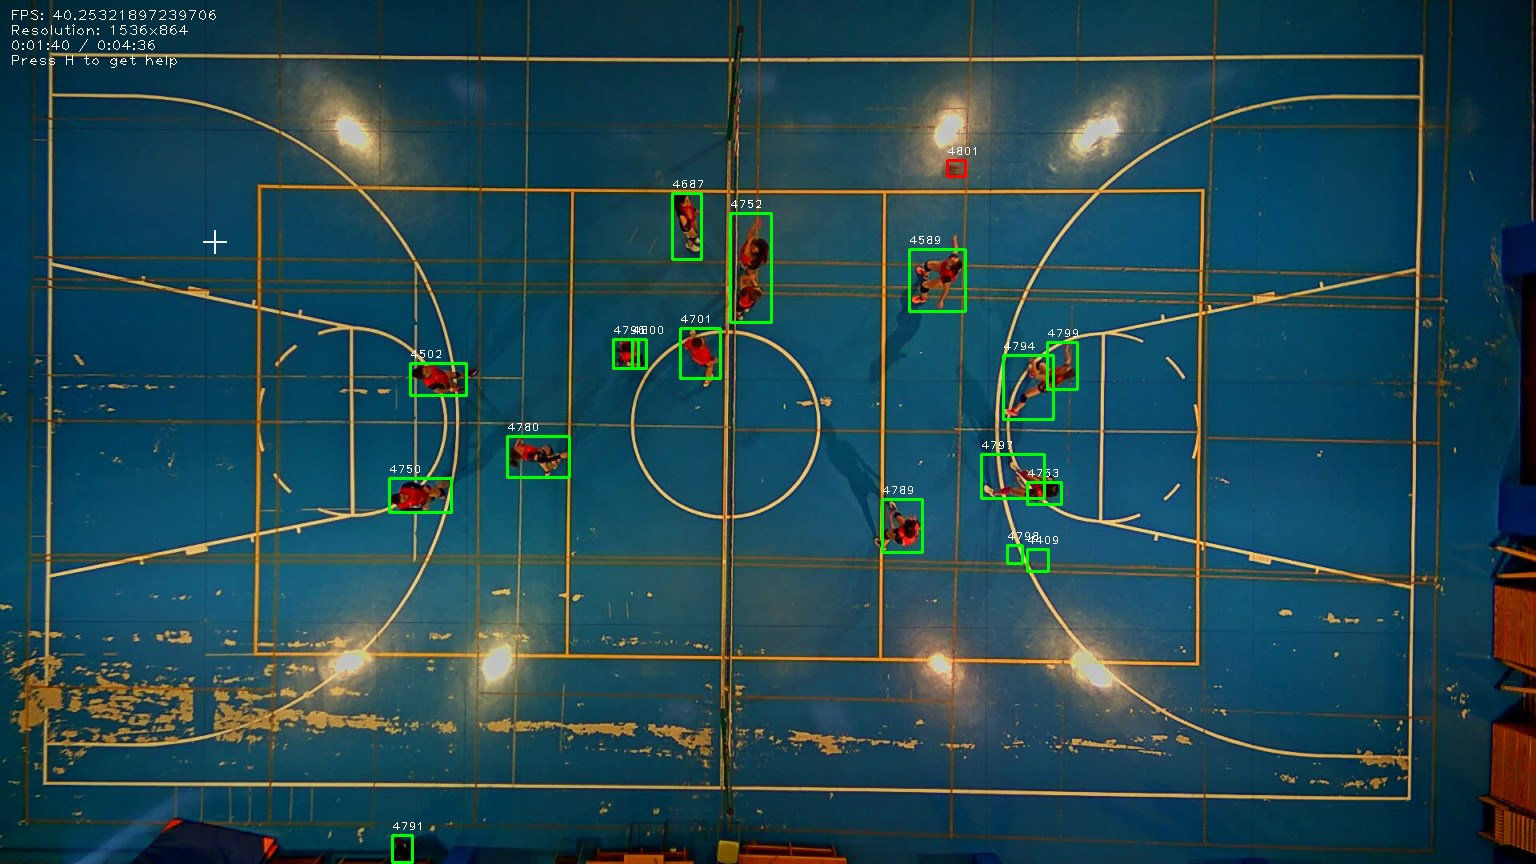
\includegraphics[width=.9\linewidth]{images/CNT}
  \caption { }
  \label{fig:CNT1b}
\end{subfigure}
\caption{Salida del algoritmo CNT: (a) Imagen binarizada del algoritmo. (b) Imagen del vídeo tras aplicar la máscara.}
\label{fig:CNT}
\end{figure}

En nuestro caso, usando este método, la reproducción del vídeo llega sobradamente a los 30 fps, con lo que puede ser útil si existe la necesidad de que la aplicación funcione en tiempo real, además de contar con un modo para paralelizar la ejecución de manera que sea incluso más rápida. Sin embargo, se aprecian problemas de ruido en la imagen binarizada, lo cual crea varios contornos falsos, como puede verse en la figura \ref{fig:CNT}.

\subsubsection*{GSOC}
GSOC fue implementado durante un \textit{Google Summer of Code}, no procede de ningún artículo, sino que parte de un algoritmo existente, LSBP. El funcionamiento de este algoritmo no tiene documentación más allá de aclarar que se basa en \textit{saliencia} de vídeo \cite{4967608}. Es un algoritmo de aprendizaje no supervisado basado en un modelo dinámico de texturas y contraste local de características.

En general, el algoritmo funciona de manera bastante robusta en lo que respecta a detectar formas en la escena, e incluso es capaz de detectar sin grandes problemas las sombras. Sin embargo, no logra detectar el balón de manera consistente, por lo que sería necesario usar algún tipo de algoritmo de tracking en conjunción con este.

\begin{figure}
\begin{subfigure}{.5\textwidth}
  \centering
  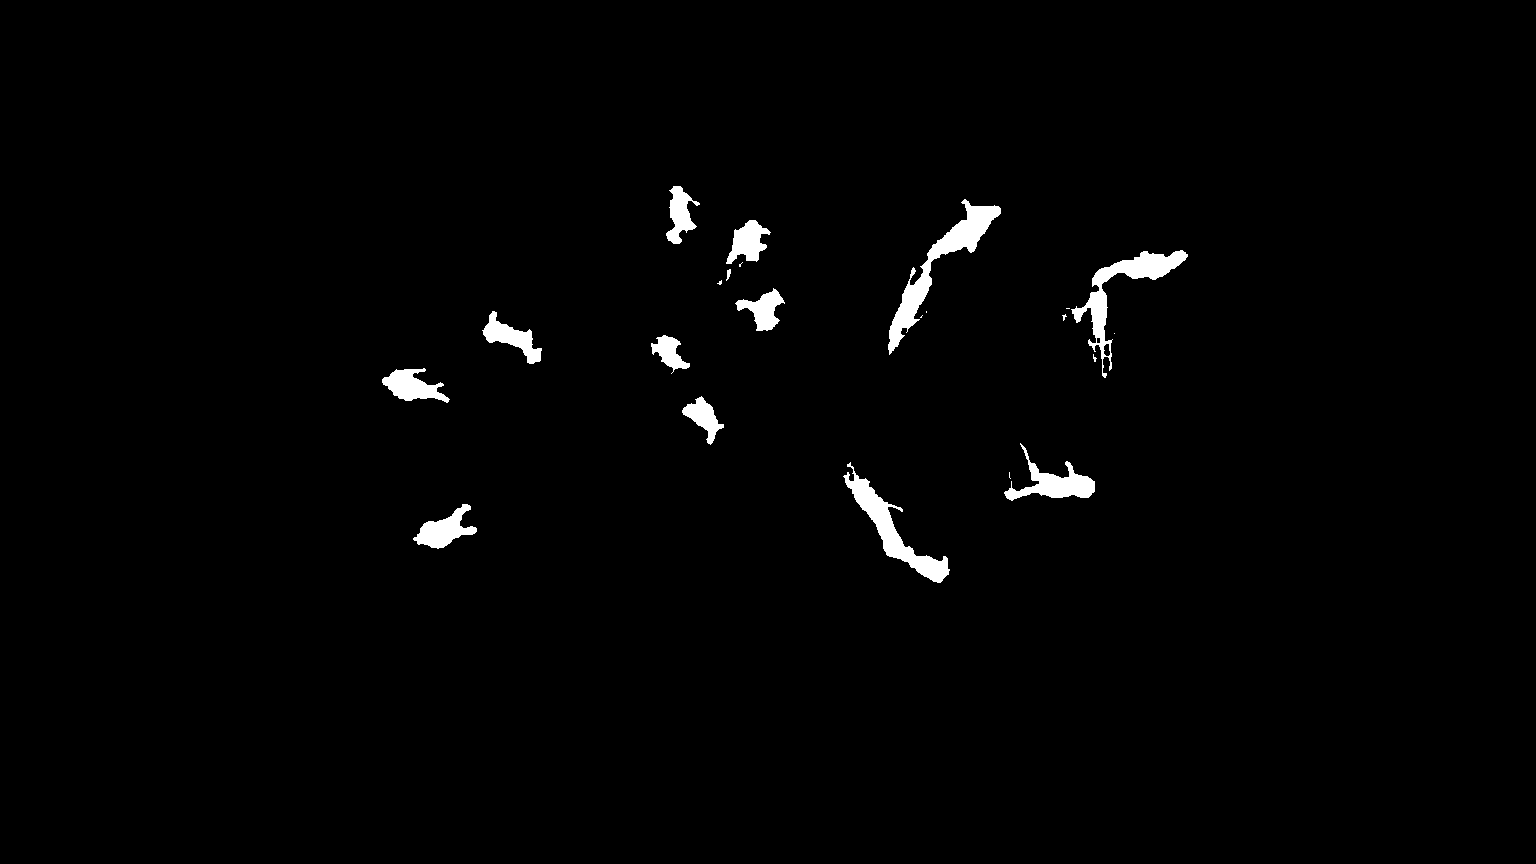
\includegraphics[width=.9\linewidth]{images/GSOCsub}
  \caption { }
  \label{fig:GSOC1a}
\end{subfigure}%
\begin{subfigure}{.5\textwidth}
  \centering
  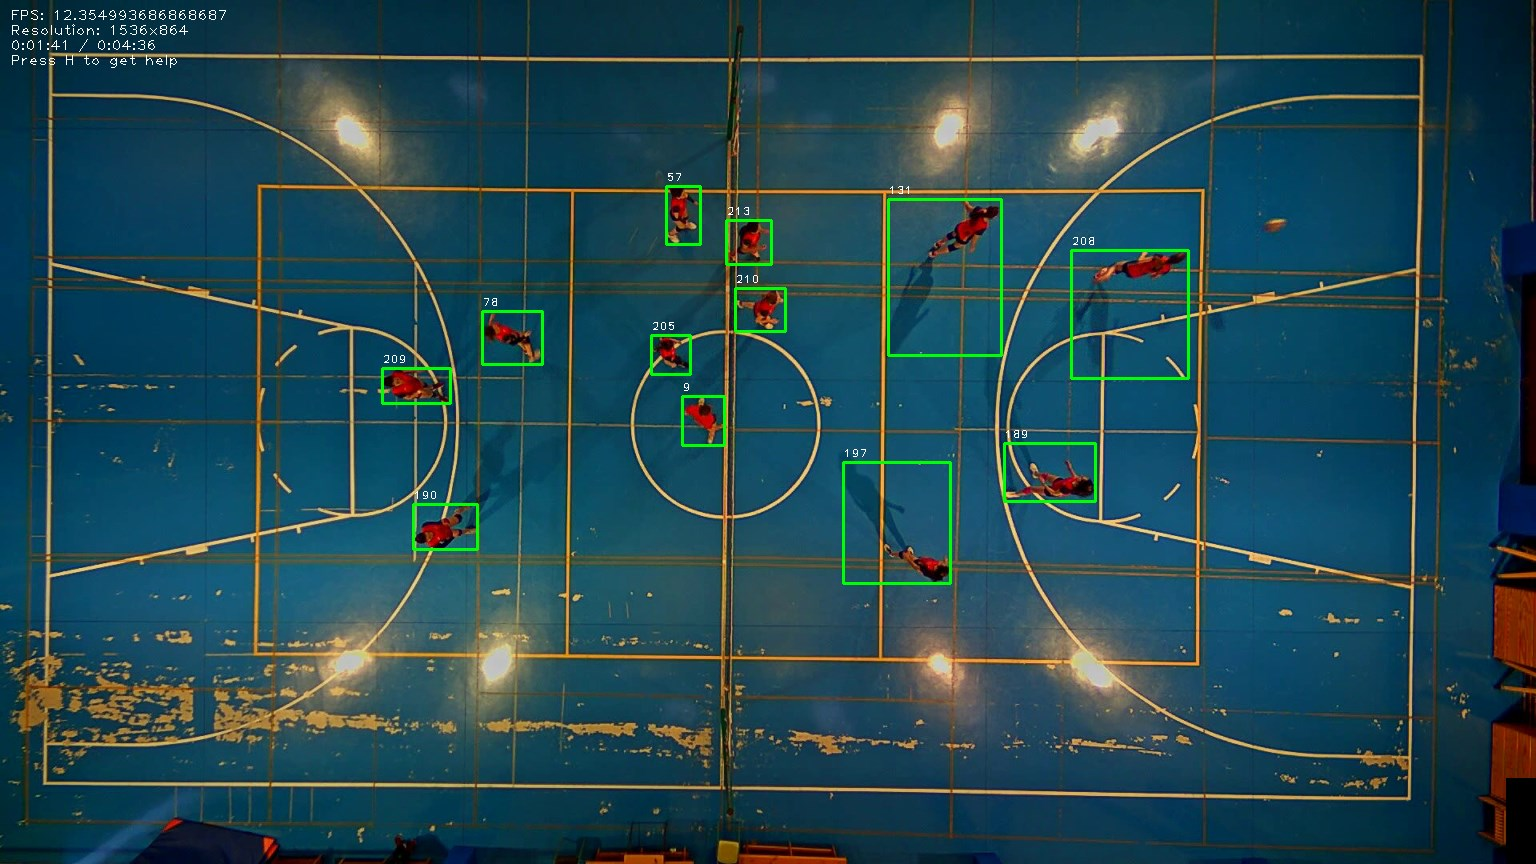
\includegraphics[width=.9\linewidth]{images/GSOC}
  \caption { }
  \label{fig:GSOC1b}
\end{subfigure}
\caption{Salida del algoritmo GSOC: (a) Imagen binarizada del algoritmo. (b) Imagen del vídeo tras aplicar la máscara.}
\label{fig:GSOC}
\end{figure}

Por otro lado, a pesar de su robustez y de que es paralelizable, el algoritmo es el más lento de los que se han probado, lo que lo hace bastante desaconsejable para aplicaciones en tiempo real.

\subsubsection*{KNN}
\begin{figure}[H]
    \centering
    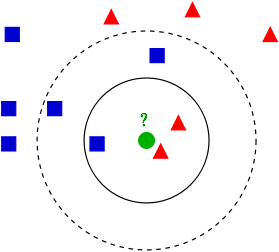
\includegraphics[width=0.3\textwidth]{images/knnejemplo}
    \caption{Ejemplo de funcionamiento de KNN en entorno bidimensional con $k=3$ en línea continua y $k=5$ en línea discontinua}
    \label{fig:knnejemplo}
\end{figure}

KNN \cite{Bishop:2006:PRM:1162264}, también conocido como método de los k-vecinos más cercanos, es un algoritmo bastante popular en reconocimiento de patrones. Es un método de clasificación supervisada no paramétrico.

\begin{figure}
\begin{subfigure}{.5\textwidth}
  \centering
  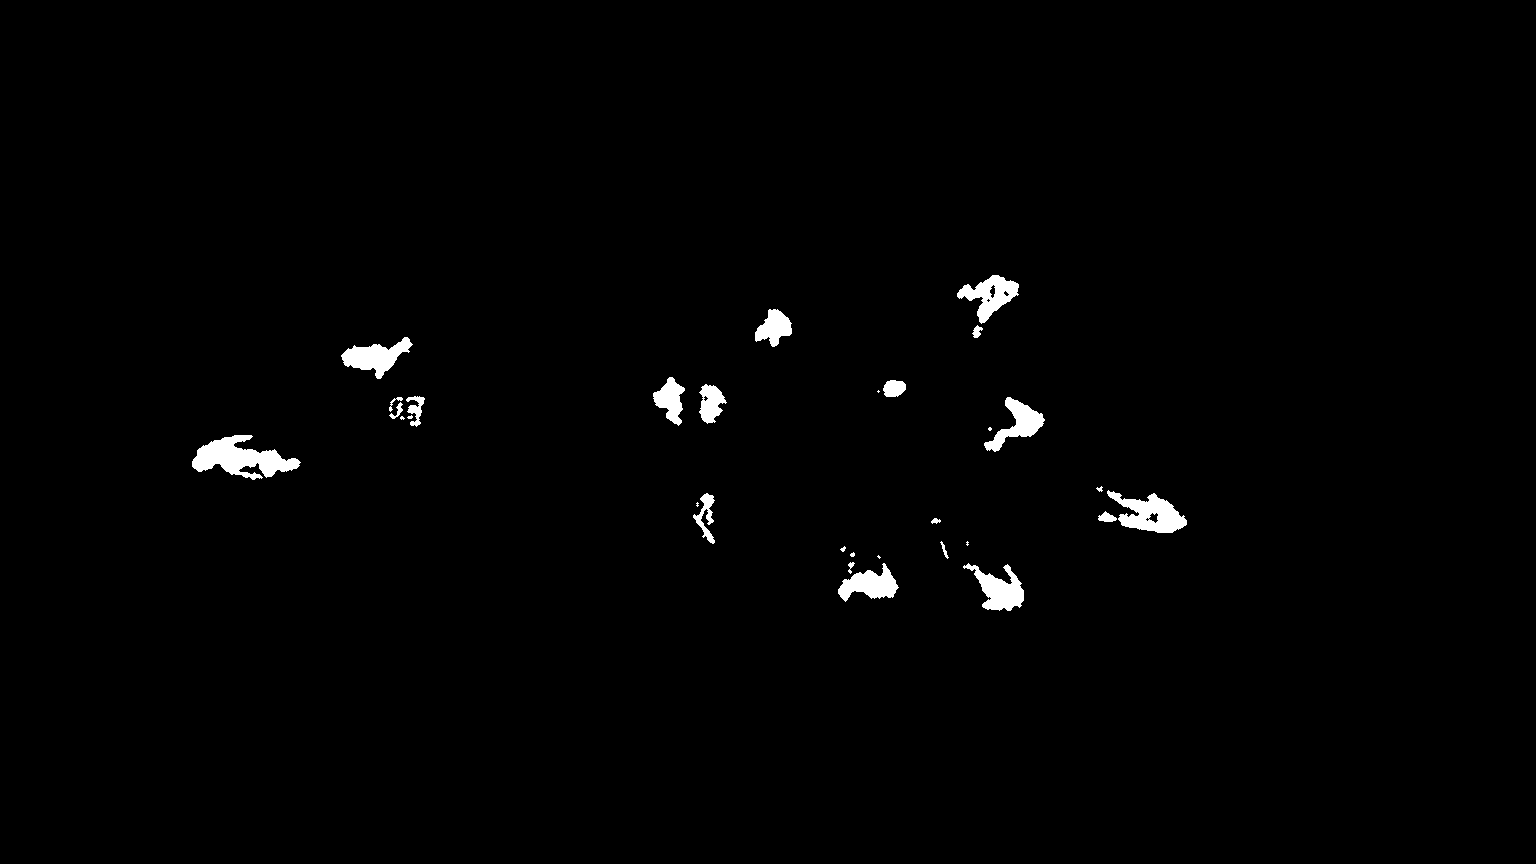
\includegraphics[width=.9\linewidth]{images/KNNsub}
  \caption { }
  \label{fig:KNN1a}
\end{subfigure}%
\begin{subfigure}{.5\textwidth}
  \centering
  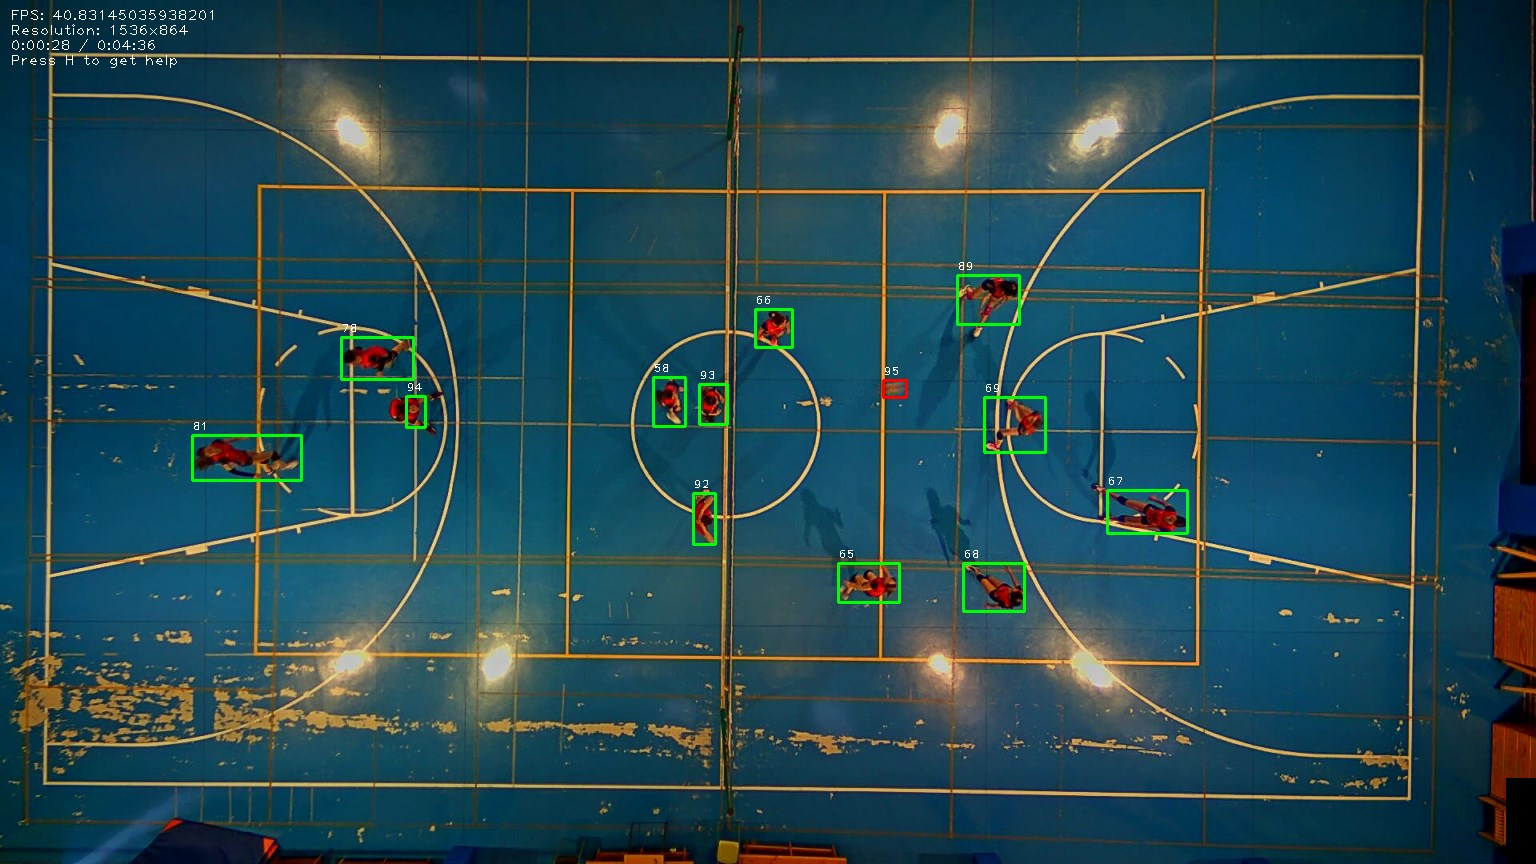
\includegraphics[width=.9\linewidth]{images/KNN}
  \caption { }
  \label{fig:KNN1b}
\end{subfigure}
\caption{Salida del algoritmo KNN: (a) Imagen binarizada del algoritmo. (b) Imagen del vídeo tras aplicar la máscara.}
\label{fig:KNN}
\end{figure}

La base del funcionamiento algoritmo es sencilla: dados unos datos etiquetados, y un punto nuevo del que no conocemos su clase, se trata de inferir a qué clase pertenece calculando las distancias a los k vecinos más cercanos. La clase del punto será la misma que tenga la mayoría de sus k vecinos más cercanos. Por ejemplo, en la figura \ref{fig:knnejemplo} podemos ver cómo el círculo verde, que es del que desconocemos su clase, tiene, con $k=3$ como vecinos 2 triángulos y 1 cuadrado, por lo que se etiquetaría como triángulo. Si por el contrario tenemos $k=5$, entonces hay 3 cuadrados y 2 triángulos como vecinos más cercanos, en cuyo caso se etiquetaría como cuadrado.

Dado que en el caso de la sustracción de fondo no tenemos datos etiquetados a priori, se debe realizar una primera estimación, por lo tanto, durante un número de frames iniciales $n$, se guardan las $n$ ternas RGB que actuarán como el modelo de fondo inicial. Estos datos se toman como si fueran fondo. A continuación, se calculan las $k$ distancias de cada pixel nuevo a los $T$ anteriores y dependiendo de las distancias, se estima la probabilidad de ser fondo o no. El modelo de fondo se va actualizando, sustituyendo vectores antiguos por vectores nuevos que se consideran fondo.

Según Zivkovic \cite{art:Zivkovic2}, se adapta el tamaño del kernel $k$ a cada pixel. En lugar de buscar un tamaño óptimo global, se incrementa para cada pixel hasta que haya una cantidad suficiente de datos. De esa forma se logran valores de $k$ grandes en áreas con un pequeño número de muestras y valores pequeños en zonas con mayor densidad. Es común usar $k=1$, pero se recomienda $k=0.1T$ para mayor robustez a valores atípicos.

\subsubsection*{Operaciones posteriores}

\begin{figure}
\begin{subfigure}{.5\textwidth}
  \centering
  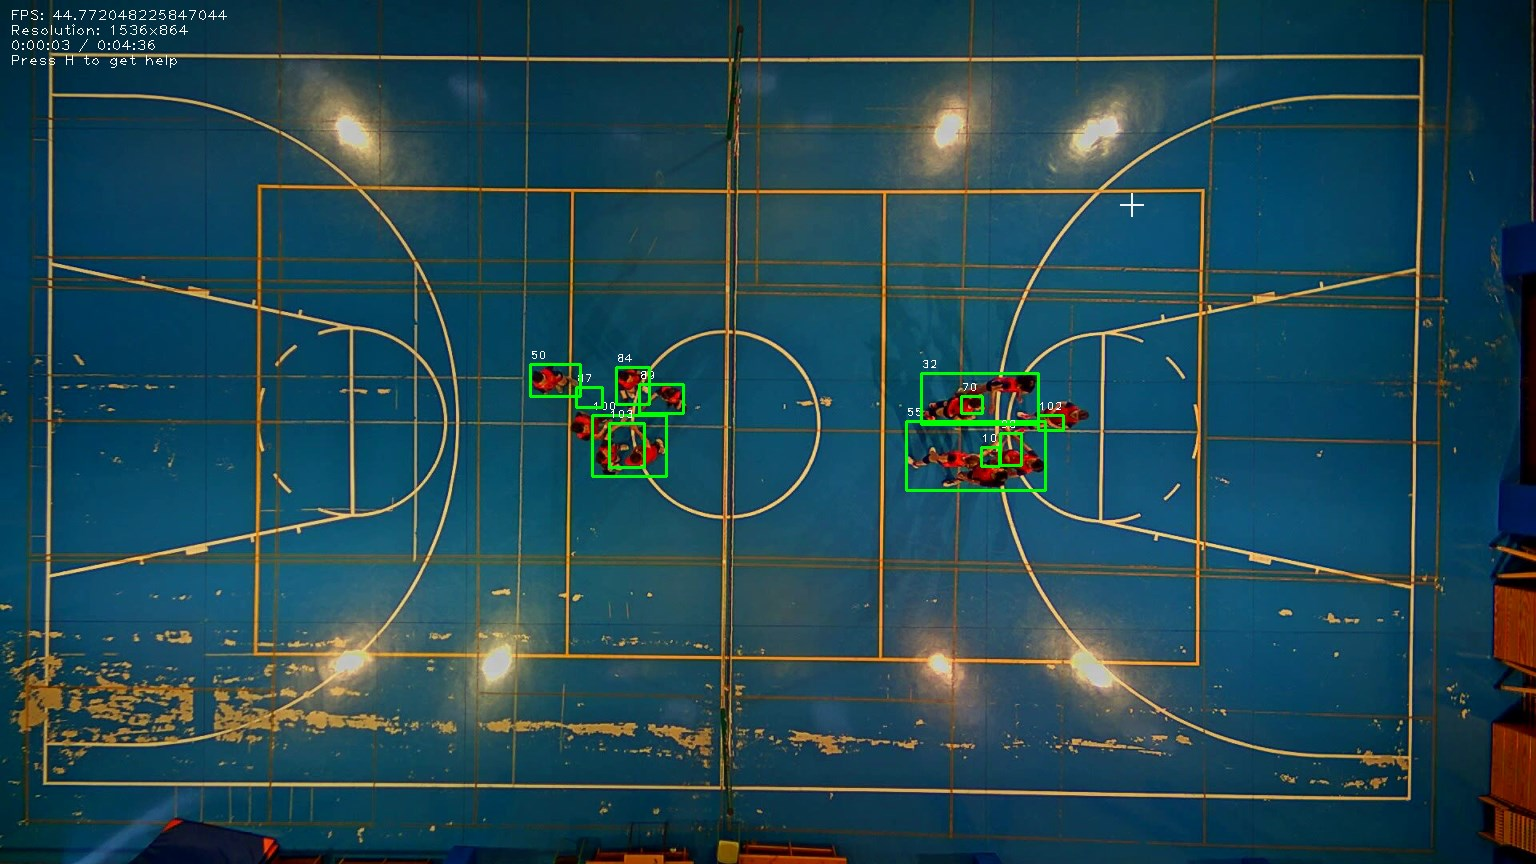
\includegraphics[width=.9\linewidth]{images/nonms}
  \caption { }
  \label{fig:nms1a}
\end{subfigure}%
\begin{subfigure}{.5\textwidth}
  \centering
  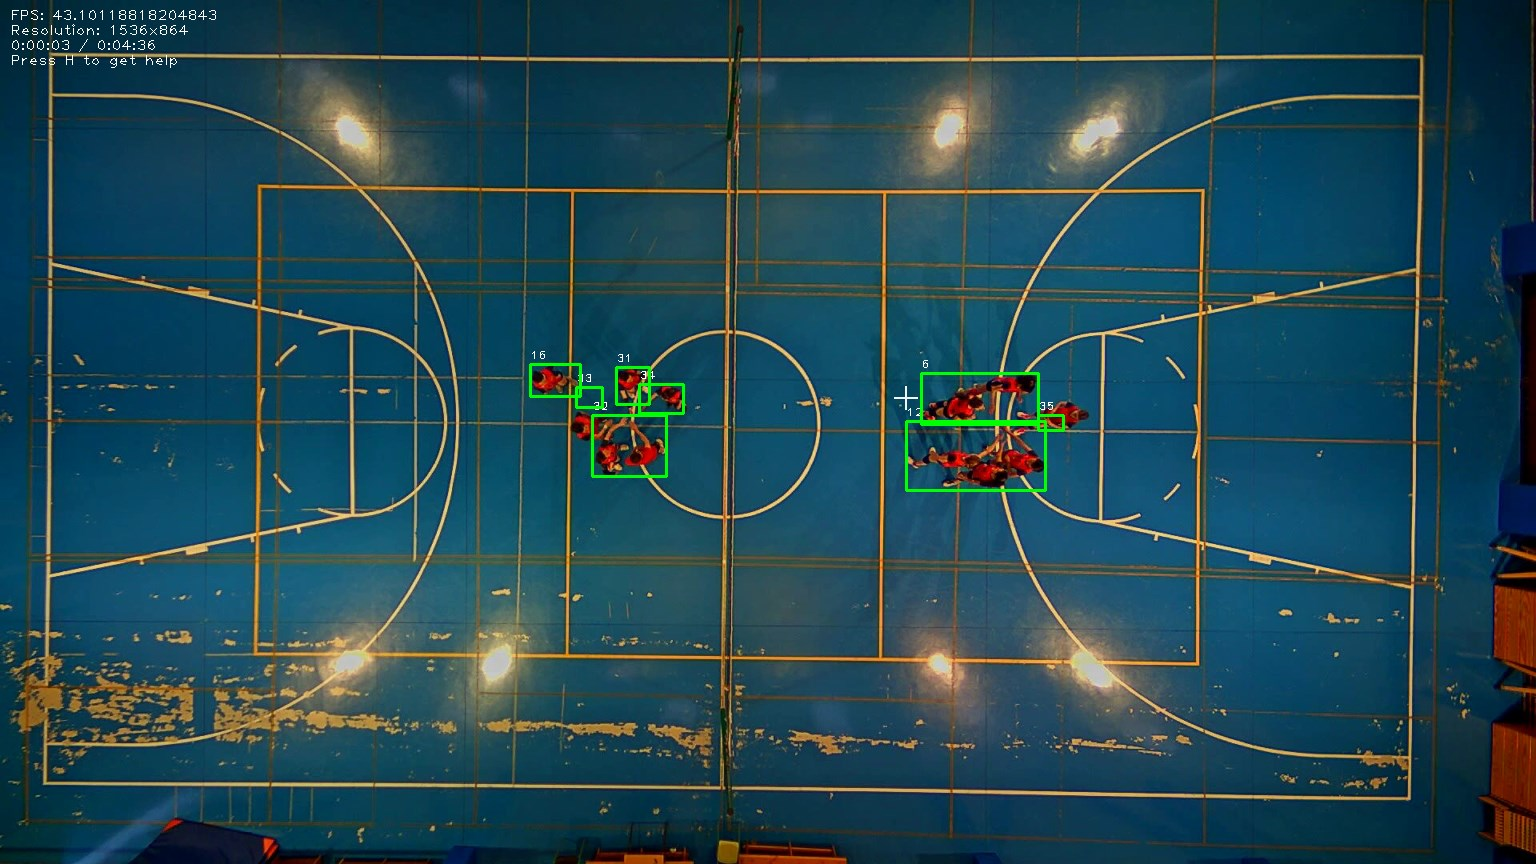
\includegraphics[width=.9\linewidth]{images/nms}
  \caption { }
  \label{fig:nms1b}
\end{subfigure}
\caption{Comparativa de la salida del vídeo antes (a) y después (b) de aplicar la operación de supresión de no máximos. }
\label{fig:nms}
\end{figure}

La primera de ellas es la \textbf{supresión de no máximos}. En ciertos momentos del vídeo, puede que no se detecte una forma de manera completa, sino que se detecta el contorno y ciertas partes separadas. Cuando esto ocurre, la imagen de salida tiene la forma que vemos en la figura \ref{fig:nms1a} donde pueden verse varios cuadrados redundantes que podrían englobarse en uno más grande. Tras aplicar la supresión de no máximos, la imagen queda como en la figura \ref{fig:nms1b}, donde puede verse que los cuadrados contenidos dentro de otros han sido suprimidos.

La segunda operación es el \textbf{test de circularidad}, el cual nos sirve para saber cuál de las formas detectadas en la imagen es el balón. Para ello, calculamos el coeficiente de circularidad $C =  \frac{4*\pi*\acute{a}rea}{per\acute{\imath}metro^2}$. Cuanto mayor sea $C$, mayor probabilidad de que la forma sea la de un círculo, es decir, la del balón. En un frame cualquiera, la forma cuyo coeficiente $C$ tenga un valor mayor de 0.6 y sea el mayor de todos los contornos detectados, se marcará en rojo en la imagen de salida, mientras que el resto se marcarán en verde.

La última de las operaciones que se realizan es el \textbf{etiquetado de los contornos} detectados. Esto será importante de cara a la salida por CSV, que será util, por ejemplo, con el fin de extraer estadísticas.

Este etiquetado no es trivial, ya que de un frame a otro, no tenemos una manera rápida de saber qué contorno del frame actual corresponde con qué contorno del anterior, porque OpenCV no nos asegura ningún tipo de orden en la salida del sustractor. Para solucionar esta problemática, en el primer frame se da una etiqueta a todos los contornos que se detecta. A partir de aquí, se aplica una técnica denominada ``matching mutuo'', en los siguientes frames se irá etiquetando en base a un emparejamiento mutuo entre los contornos, calculando una matriz de distancias de todos los contornos entre sí. 

Una vez calculada esta matriz, si para un contorno $c$, su más cercano es otro contorno $k$ y si para $k$ el más cercano es $c$, esto quiere decir que son el mismo contorno. En caso de quedar contornos sin pareja después de esto, simplemente se les da una etiqueta nueva.

\subsubsection*{Comparativa entre algoritmos}

Ahora tendremos que seleccionar de entre todos los algoritmos anteriores el que mejor convenga a nuestros objetivos, teniendo en cuenta el coste computacional de cada uno, así como su desempeño a la hora de estimar el fondo.

El primer apartado a valorar será el rendimiento en frames por segundo (FPS) de cada algoritmo con distintos tamaños de imagen. Cabe aclarar que la cifra de FPS que aparece en la tabla no se mantiene constante sino que es un promedio de las cifras observadas durante la ejecución. Suponiendo que la escala 1 de imagen es la resolución original, 1920x1080, los resultados obtenidos, usando un Intel i7 6700k para procesar, son los que aparecen en la figura \ref{fig:fps}.

% \begin{table}
%     \centering
%     \begin{tabular}{| l | c | c | c |}
%     \hline
%     \textbf{Método} & \textbf{FPS a escala 1} & \textbf{FPS a escala 0.8} & \textbf{FPS a escala 0.6}\\ \hline
%     Diferencia de frames & 40 (25 ms) & 51 (19 ms) & 68 (14 ms) \\ \hline
%     MOG & 15 (66 ms) & 23 (43 ms) & 37 (27 ms) \\ \hline
%     MOG2 & 28 (35 ms) & 36 (27 ms) & 52 (19 ms) \\ \hline
%     GMG & 10 (100 ms) & 15 (66 ms) & 24 (41 ms) \\ \hline
%     CNT & 30 (33 ms) & 41 (24 ms) & 55 (18 ms)\\ \hline
%     KNN & 32 (31 ms) & 40 (25 ms) & 56 (17 ms)\\ \hline
%   \end{tabular}
%   \caption{}
%   \label{tab:1}
% \end{table}

\begin{figure}
    \centering
    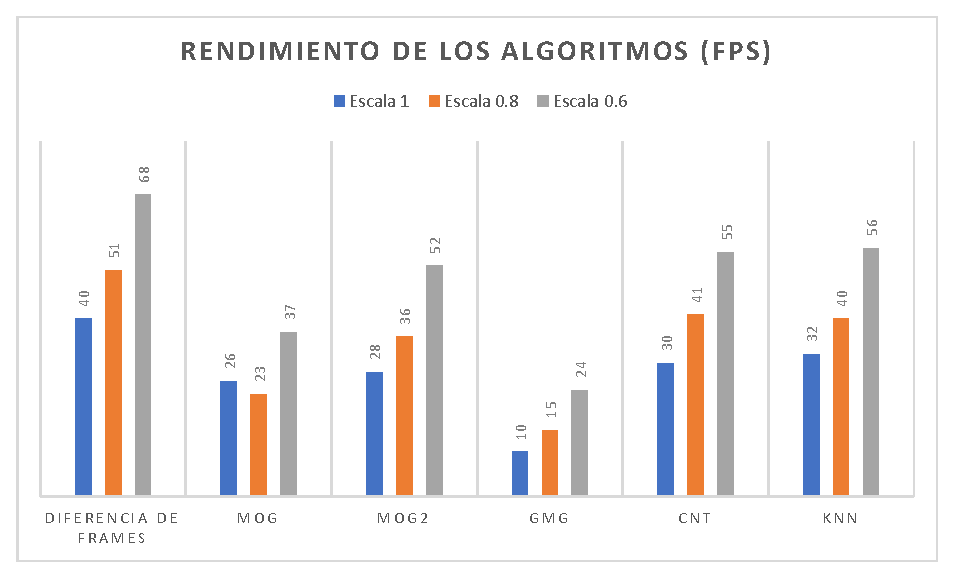
\includegraphics[width=0.7\textwidth]{images/plotFPS}
    \caption{Estadísticas de rendimiento en FPS de los algoritmos con distintos tamaños de imagen (sobre CPU i7-6700k).}
    \label{fig:fps}
\end{figure}


Podemos ver que CNT y KNN son los dos mejores en lo que a velocidad se refiere, con valores de fps muy parejos, seguidos por MOG2. Por otro lado, GMG es de todos los métodos el más lento con diferencia.

Como se ha visto antes, MOG2 es sensiblemente más rápido que MOG debido a que se adapta el número de mezclas por zonas de la imagen, haciendo que el procesamiento de cada frame sea más rápido si se necesitan menos mezclas gaussianas.

Mención aparte merece el método de resta de frames, ya que, aunque es el que mejores números tiene, su detección no es especialmente buena debido a la sensibilidad a cambios de iluminación, por lo que, a pesar de su buena velocidad, seguimos manteniéndolo como descartado.

CNT es también otro descarte a pesar de estar entre los tres más rápidos, debido a su falta de estabilidad y robustez a la hora de detectar formas, que lo hace poco útil en nuestro caso concreto. 

\begin{figure}
\begin{subfigure}{.5\textwidth}
  \centering
  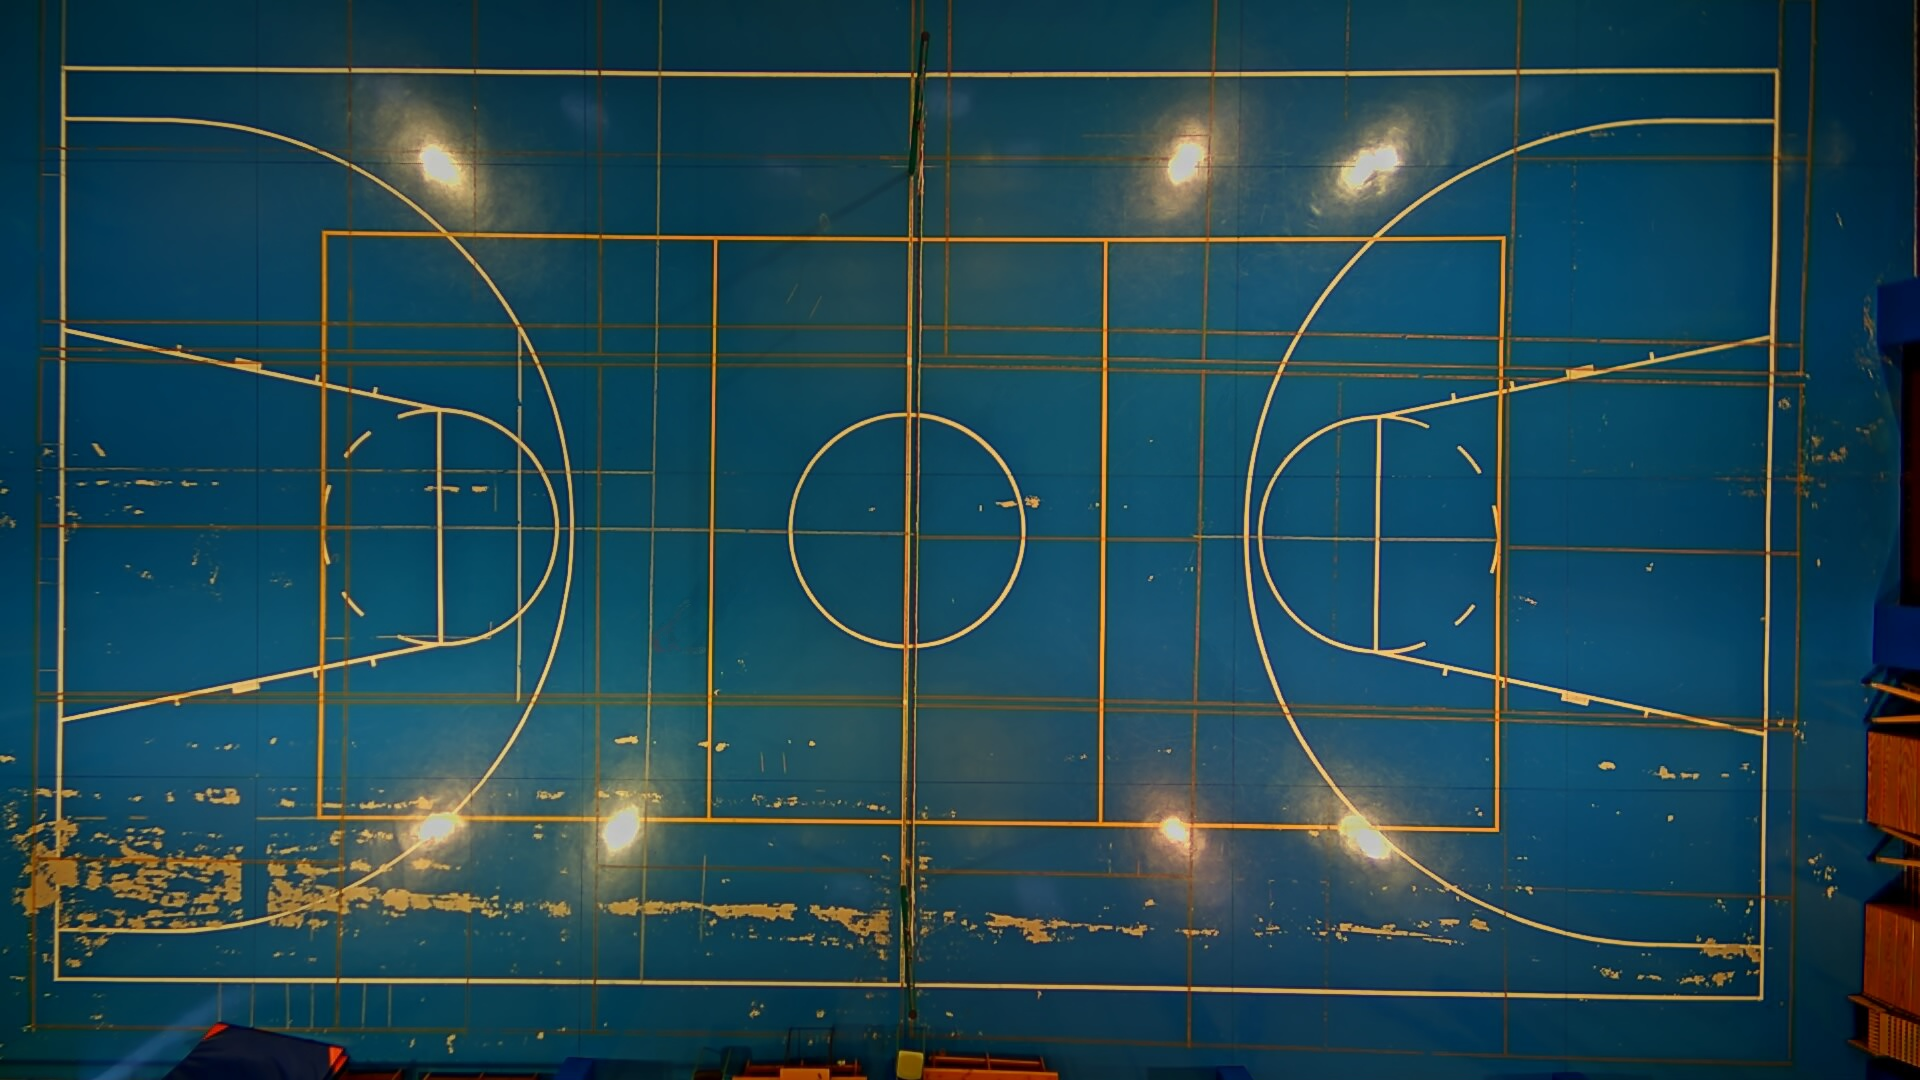
\includegraphics[width=.9\linewidth]{images/modeloMOG}
  \caption { }
  \label{fig:modelos1a}
\end{subfigure}%
\begin{subfigure}{.5\textwidth}
  \centering
  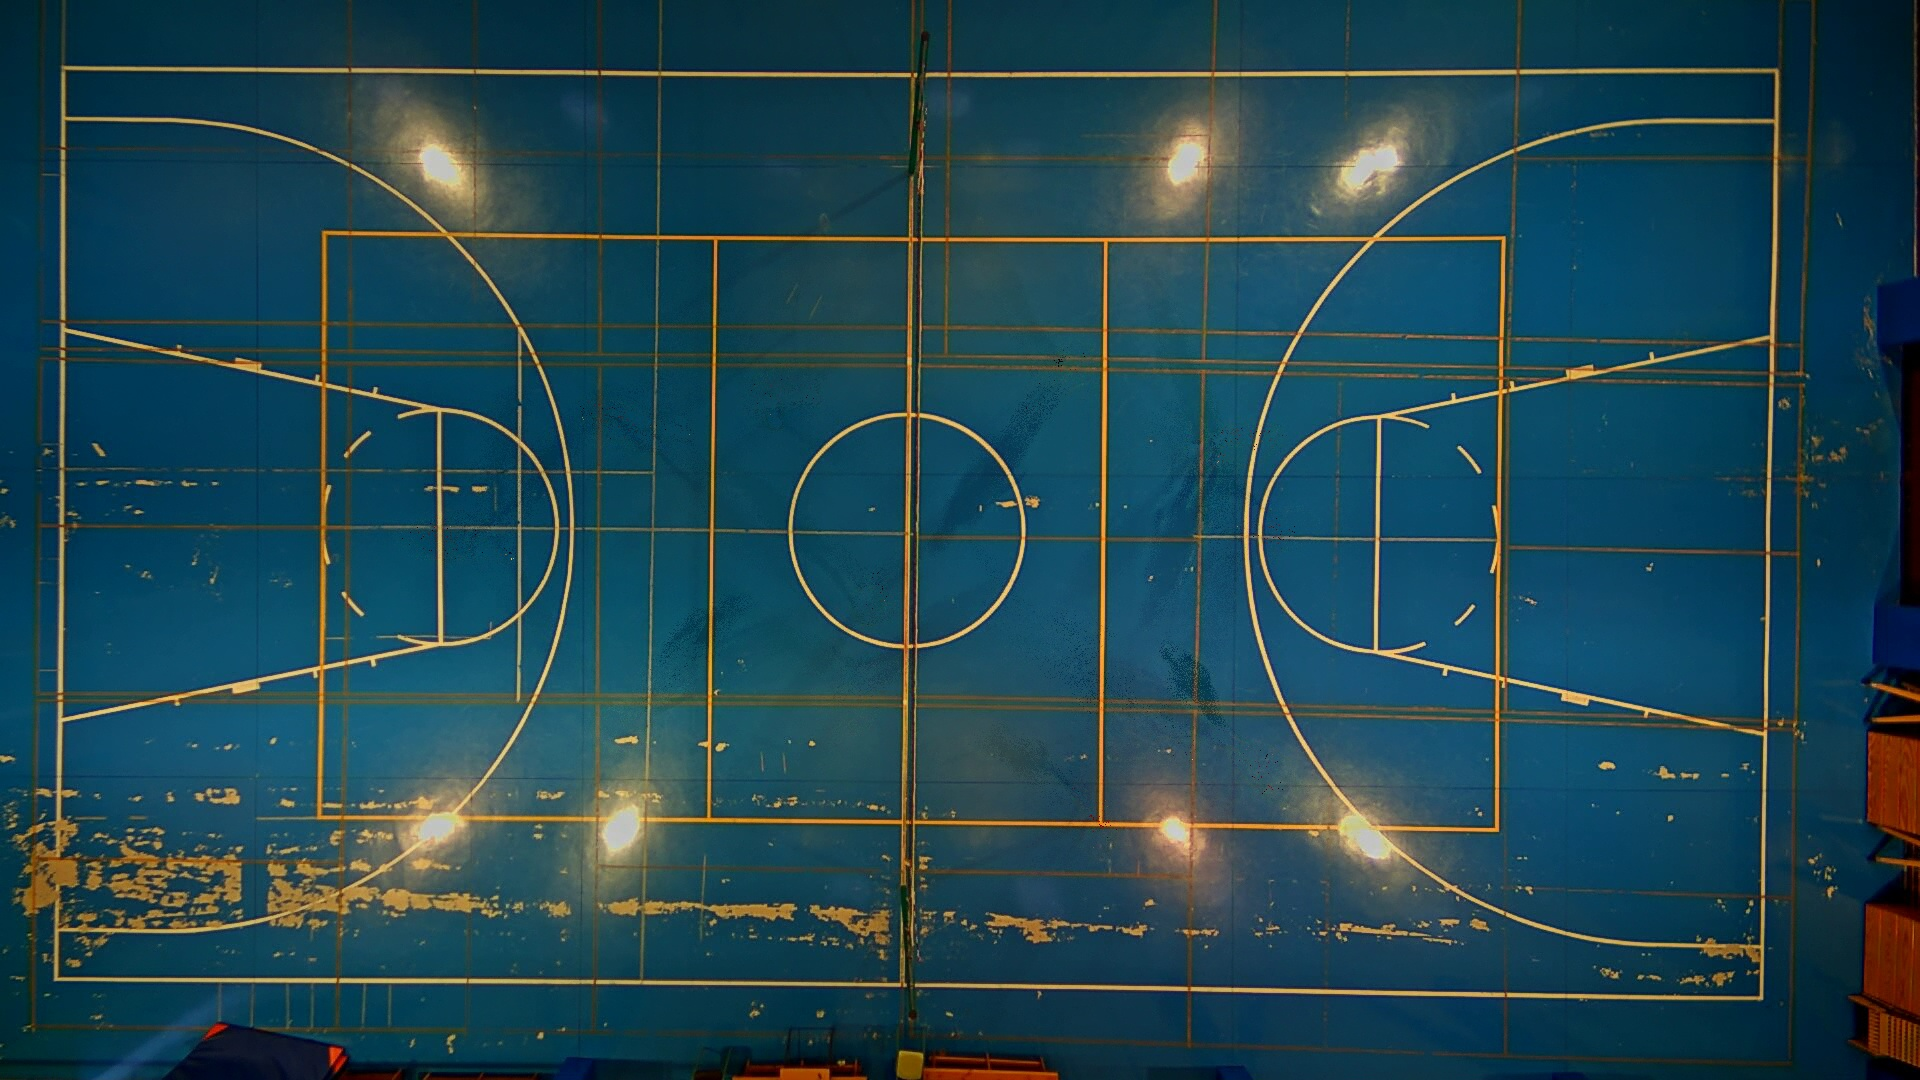
\includegraphics[width=.9\linewidth]{images/modeloKNN}
  \caption { }
  \label{fig:modelos1b}
\end{subfigure}
\caption{Comparativa entre los modelos de fondo finales de MOG2 (a) y KNN (b) tras un vídeo de un set completo. }
\label{fig:modelos}
\end{figure}

Con lo cual, nos toca decidir entre MOG2 y KNN, que son los dos candidatos que nos quedan atendiendo a la velocidad de ambos. Ambos tienen una detección muy parecida, pero MOG2 es ligeramente superior a la hora de estimar el modelo de fondo (En la figura \ref{fig:modelos} se puede ver que el modelo de MOG2 es más limpio). También es mejor MOG2 en ciertas ocasiones a la hora de detectar sombras. Por estos motivos, sumados a que la velocidad no es un requisito principal del trabajo, se usará MOG2 como método principal para sustracción de fondo, si bien el software final permite el uso de cualquier otro método de los expuestos a fin de mantener todas las posibilidades a disposición del usuario.

\subsection{Seguimiento}
Otra manera mediante la que podemos detectar a las jugadoras y al balón es el seguimiento o \textit{tracking}. Cabe aclarar que no necesariamente es excluyente el uso de esta técnica con el de sustracción de fondo, sino que puede servir para complementar a esta en ciertos objetos que el sustractor de fondo no detecte correctamente.

Nuevamente, OpenCV pone a nuestra disposición 2 algoritmos de seguimiento: Mean Shift y CAMShift. El módulo colaborativo añade otros cuantos más. Al igual que en el apartado anterior, se usará la programación orientada a objetos para crear una jerarquía de clases que haga sencilla la selección del algoritmo a usar, proporcionando una interfaz común al programar.

Los algoritmos de seguimiento que proporciona el módulo colaborativo de OpenCV son Boosting, MIL, Median Flow y TLD, y fueron los primeros que se probaron e implementaron. Los resultados no fueron muy satisfactorios con ninguno de ellos, y la diferencia en calidad de estos algoritmos no justifica el coste en velocidad que suponen respecto a Mean Shift y CAMShift.

\begin{figure}
    \centering
    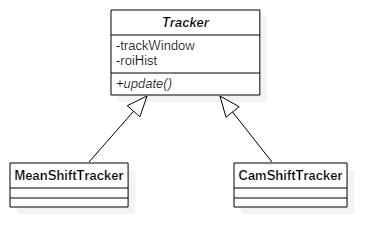
\includegraphics[width=0.35\textwidth]{images/trackers}
    \caption{Estructura de clases de los algoritmos de \textit{tracking}.}
    \label{fig:trackers}
\end{figure}

Tras descartar los anteriores métodos, se implementaron los métodos de Mean Shift y CAMShift. Como se ha dicho antes, se ha utilizado una estructura de clases parecida a la de los sustractores de fondo (figura \ref{fig:trackers}) con el mismo objetivo: dar una interfaz común a todas las clases que haga sencillo el seleccionar el algoritmo que se quiera utilizar antes de ejecutar el programa.

\subsubsection*{Mean Shift}
Mean Shift es una técnica de análisis de espacios de características no paramétrica que consiste en localizar los máximos de una función de densidad, es decir, es un algoritmo de búsqueda de modas. Fue presentada por Fukunaga y Hostetler en 1975 \cite{1055330}. Entre sus aplicaciones se encuentran procesamiento y segmentación de imágenes (figura \ref{fig:clustering}) y, por supuesto, el tema que nos ocupa: el seguimiento o \textit{tracking}.

\begin{figure}
    \centering
    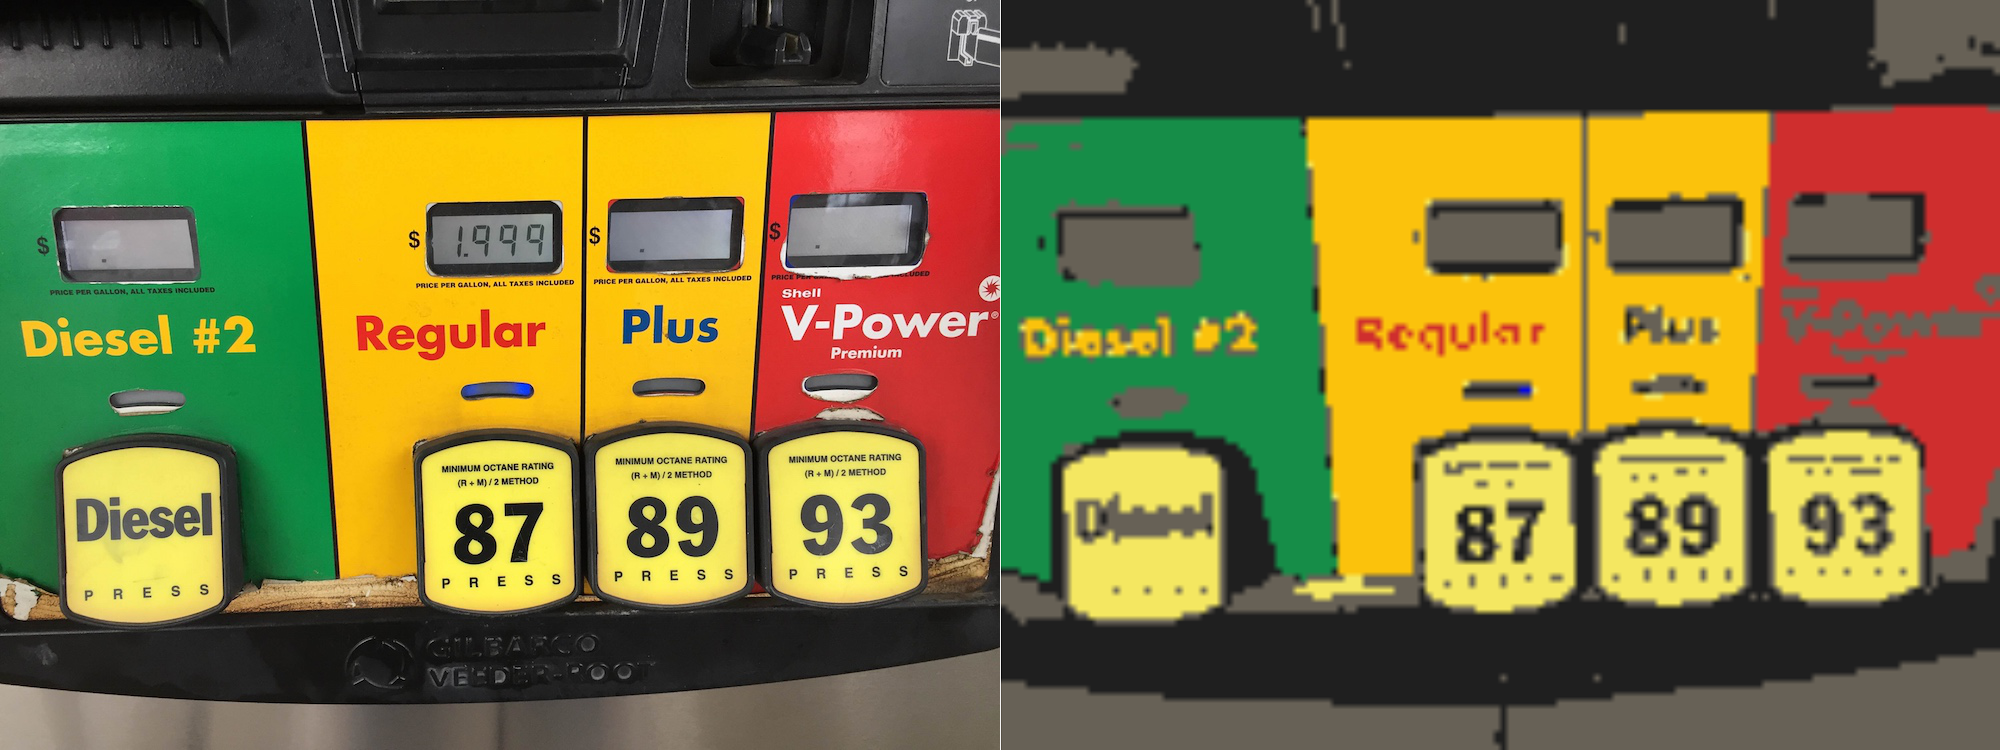
\includegraphics[width=0.6\textwidth]{images/clustering}
    \caption{Ejemplo de aplicación de Mean Shift para clustering.}
    \label{fig:clustering}
\end{figure}

El algoritmo de Mean Shift, como se ha dicho, tiene como objetivo la búsqueda de máximos de una función de densidad dada. Para hacerlo, se calcula de manera iterativa a partir de una estimación $x$, conocida como ventana. Una vez proporcionada una ventana al algoritmo, se calculan los pesos de todos los puntos de alrededor de $x$ mediante una función $K$, que normalmente suele tener la forma $K(x_i-x) = e^{-c||x_i-x||^2}$. La media pesada de la densidad en la ventana es:
\[
  m(x) = \frac{\sum_{x_i\in N(x)}K(x_i-x)x_i}{\sum_{x_i\in N(x)}K(x_i-x)}
\]
siendo $N(x)$ el conjunto de vecinos en $x$.

La diferencia $m(x)-x$ es lo que se llama \textit{mean shift} (literalmente: desplazamiento de media) en el trabajo de Fukunaga y Hostetler. En la siguiente iteración se hace $x= m(x)$ y se repite hasta que $m(x)$ converge al mismo valor, con un cierto margen de error.

Ahora bien, en el caso del seguimiento, el algoritmo se adapta a esta aplicación concreta. La ventana inicial es una región de interés de la imagen, a la cual se le calcula el histograma. En cada frame del vídeo, se calcula la retroproyección, es decir, la probabilidad de que un pixel de la imagen pertenezca a la distribución que describe el histograma inicial. Una vez calculado esto, se calcula, iterativamente, el centro de masas de los puntos localizados dentro de la ventana. Como se ha dicho antes, el algoritmo converge cuando el centroide calculado coincide con el centro de la ventana con un cierto margen de error. En la figura \ref{fig:meanshiftopencv} puede verse un diagrama de cómo se mueve la ventana en iteraciones consecutivas, hasta llegar al centro de masas.

\begin{figure}
    \centering
    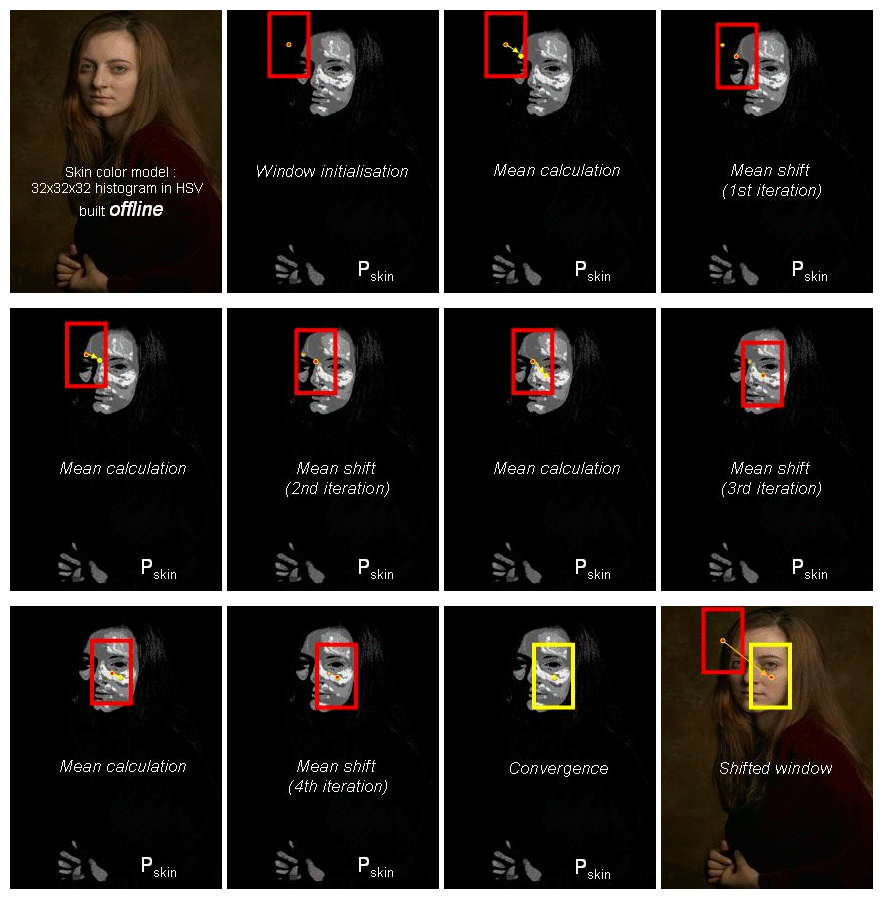
\includegraphics[width=0.65\textwidth]{images/meanshift}
    \caption{Diagrama donde puede verse el funcionamiento de Mean Shift iteración a iteración \cite{wiki:meanshift}.}
    \label{fig:meanshiftopencv}
\end{figure}


Entre las ventajas de Mean Shift se encuentra su capacidad para manejar y adaptarse a distintos espacios de características, además de, en el caso de la segmentación, que no es necesario dar un número de clusters de datos, sino que el algoritmo es capaz de hallarlos por sí mismo. Sin embargo, es un algoritmo más bien lento aunque fácilmente paralelizable, y, en el caso del seguimiento, dado que el tamaño de la ventana es constante, puede tener problemas en caso de que algún objeto de la escena cambie de tamaño (se acerque o bien se aleje, como veremos en la figura \ref{fig:ejemplos1a})

\subsubsection*{CAMShift}

CAMShift es una versión adaptativa del algoritmo anterior propuesta por Gary Bradski \textit{et al.} \cite{art:camshift}. Básicamente, este método soluciona la falta de adaptabilidad de la ventana de Mean Shift. Para ello, se aplica en cada frame Mean Shift de la misma manera que se ha expuesto en el apartado anterior. La diferencia es que en este caso, tras la aplicación de Mean Shift, se calculan $M_{00}$, $M_{20}$ y $M_{02}$, definidos por:
\[
  M_{00} = \sum_x \sum_y I(x,y) ; M_{20} = \sum_x \sum_y x^2 I(x,y) ; M_{02} = \sum_x \sum_y y^2 I(x,y)
\]

Siendo $I(x,y)$ la probabilidad en la posición $(x,y)$. Con estos valores se calculan los parámetros de la nueva ventana: orientación $\theta$, longitud $l$ y anchura $w$. Sea

\[
a = \frac{M_{20}}{M_{00}} - x_c^2 ; b = 2(\frac{M_{11}}{M_{00}}-x_cy_c) ; c = \frac{M_{02}}{M_{00}} - y_c^2
\]
La nueva ventana puede calcularse como
\begin{gather*}
  \theta = \frac{\arctan \frac{2b}{a-c}}{2} \\
  l = \sqrt{\frac{(a+c)+\sqrt{b^2+(a-c)^2}}{2}} \\
  w = \sqrt{\frac{(a+c)-\sqrt{b^2+(a-c)^2}}{2}}
\end{gather*}

El resto del método es exactamente igual que Mean Shift, se hace uso de un histograma y retroproyecciones para calcular el centro de la ventana. Por ello, el resultado obtenido es igualmente bueno con la ventaja de que se adapta a cambios de tamaño en los objetos de la escena. Sin embargo, CAMShift es ligeramente más costoso de procesar, debido a los cálculos necesarios para hallar las medidas de la ventana. En la figura \ref{fig:camshiftopencv} podemos ver iteración a iteración cómo CAMShift se adapta a una cara en el caso de una imagen estática.

\begin{figure}
    \centering
    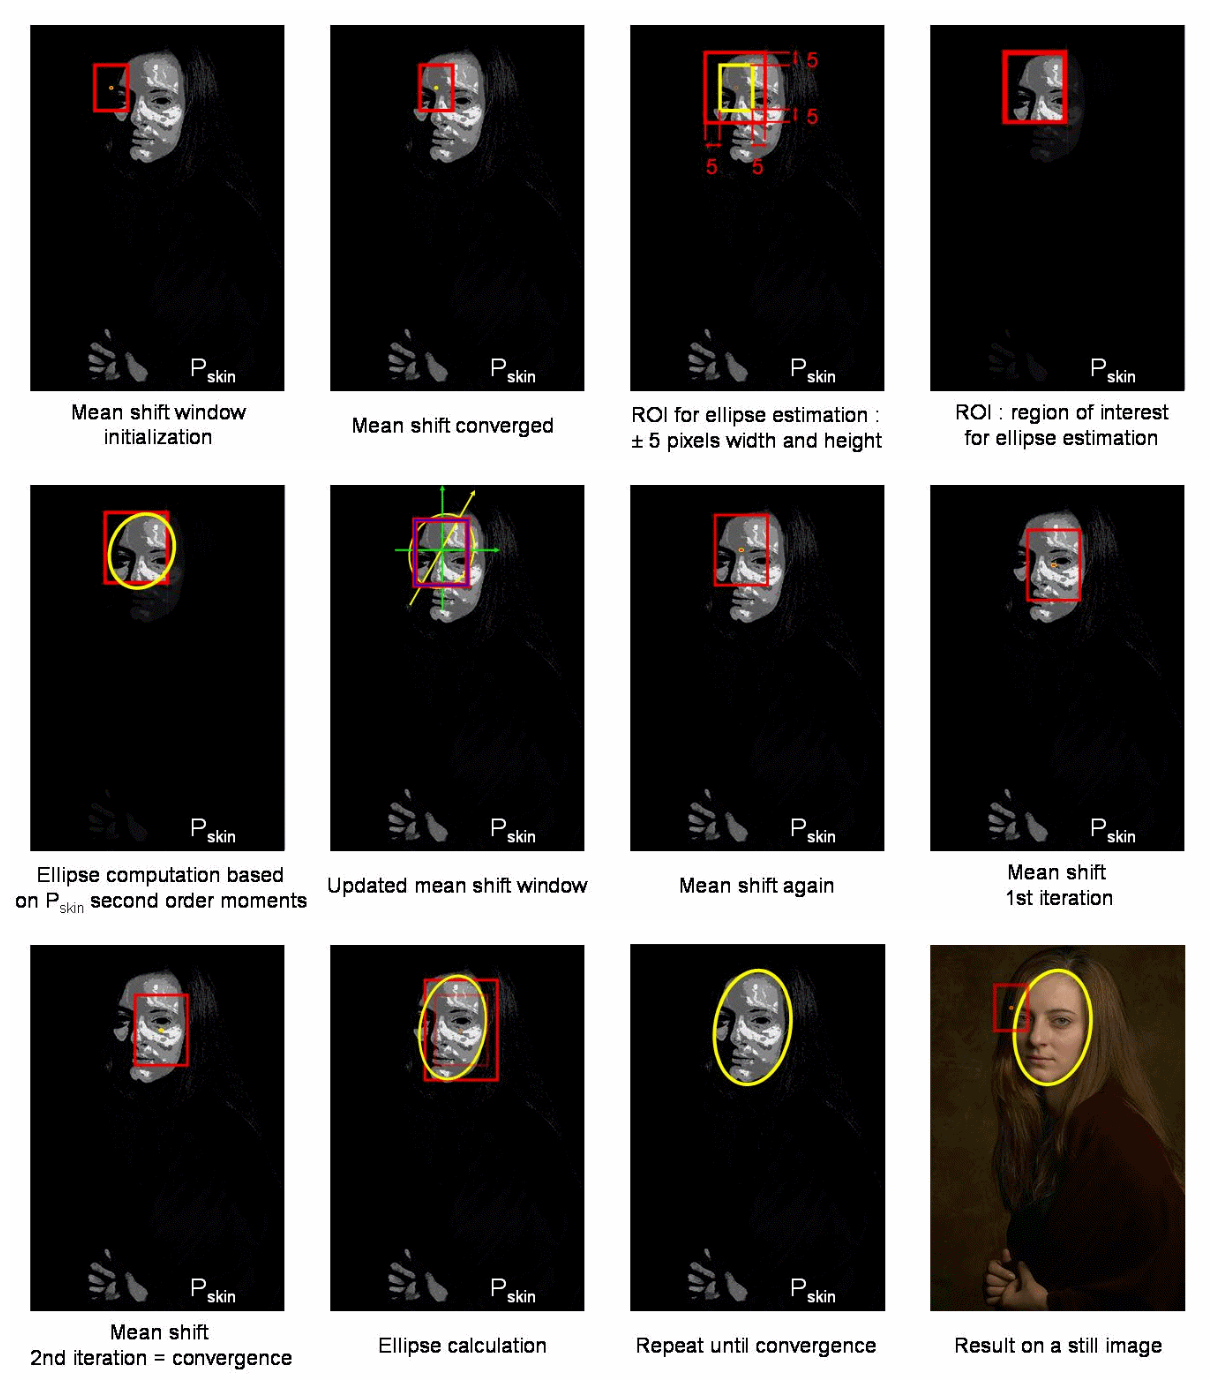
\includegraphics[width=0.7\textwidth]{images/camshift}
    \caption{Diagrama de funcionamiento de CAMShift iteración a iteración \cite{wiki:camshift}.}
    \label{fig:camshiftopencv}
\end{figure}

Para nuestro caso, debemos ser extremadamente cuidadosos a la hora de seleccionar la ventana inicial, a fin de evitar que en caso de que dos jugadoras se acerquen, sus ventanas pasen a englobar a ambas.

\subsubsection*{Comparativa y selección}

\begin{figure}
  \begin{subfigure}{.5\textwidth}
    \centering
    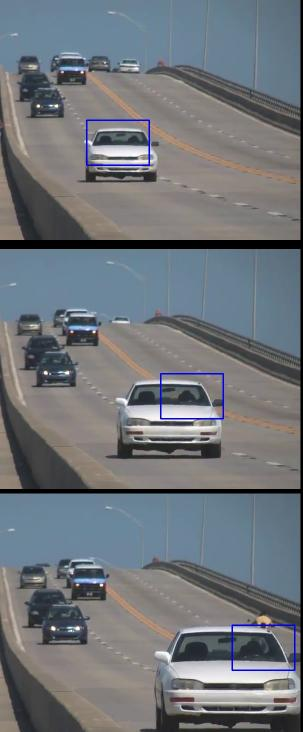
\includegraphics[width=.45\textwidth]{images/cochemeanshift}
    \caption{}
    \label{fig:ejemplos1a}
  \end{subfigure}
  \begin{subfigure}{.4\textwidth}
    \centering
    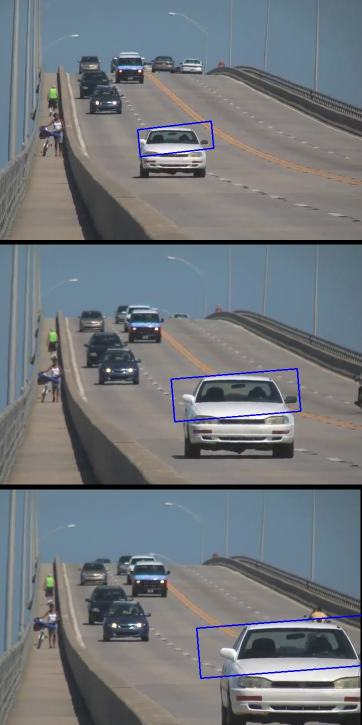
\includegraphics[width=0.65\textwidth]{images/cochecamshift}
    \caption{ }
    \label{fig:ejemplos1b}
  \end{subfigure}
  \caption{Ejemplos de tracking usando Mean Shift y CAMShift (a) Usando Mean Shift (b) Usando CAMShift.}
  \label{fig:ejemplos}
\end{figure}

En la mayoría de entornos, la adaptabilidad de CAMShift lo hace superior en lo que a seguimiento se refiere. Esta adaptabilidad puede verse en la figura \ref{fig:ejemplos}, que compara la salida de ambos métodos en el mismo vídeo, y puede verse que la ventana de CAMShift se adapta perfectamente al cambio de tamaño del coche en la imagen. Sin embargo, esta mejora tiene un pequeño coste computacional. 

En el caso que nos ocupa, dado que la cámara es fija, los objetos no se alejan ni acercan a ella, con la salvedad de cuando el balón asciende, que aun con todo, no resulta un problema para su seguimiento. Además, CAMShift es muy sensible a acercamientos entre jugadoras: incluso aunque sus ventanas no lleguen a solaparse, es frecuente que el algoritmo agrande las ventanas para hacerlas englobar a las dos jugadoras y nunca llega a recuperarse de esa situación para volver a enmarcar solamente a una de ellas. Debido a esto, y para evitar un coste computacional adicional que no nos resultaría especialmente útil, se ha optado por Mean Shift como algoritmo de seguimiento por defecto, aunque como en el caso de los algoritmos de sustracción de fondo, se permite el uso de CAMShift en el software final.

A la hora de analizar los FPS obtenidos con cada uno de los algoritmos, debe aclararse antes cómo se actualiza un frame en la implementación de OpenCV. En ambos casos debe pasársele siempre a la función de actualización el frame completo junto con una ventana que es la ventana resultante del frame anterior. Esta implementación tiene una desventaja, y es que la retroproyección se calcula de todo el frame, aunque luego se busca la nueva ventana (es decir, el objeto que se esta siguiendo) en los alrededores de la anterior. Para evitar hacer un cálculo en todo el frame de manera innecesaria, proponemos una solución que consiste en usar una sección de la imagen, algo trivial de obtener mediante la sintaxis de Python. Esta sección corresponde a los alrededores de la ventana, y por ser de un tamaño más reducido, se agiliza la computación de cada frame.

\begin{table}
  \centering
  \begin{tabular}{|l|c|l|}\hline
  \textbf{Método} & \multicolumn{1}{m{4cm}|}{\textbf{FPS usando imagen completa}}&  \multicolumn{1}{m{4cm}|}{\textbf{FPS usando secciones de imagen}}\\\hline
  Mean Shift & 15 (66 ms) & 32 (31 ms) \\\hline
  CAMShift & 13 (76 ms)& 30 (33 ms)\\\hline
  \end{tabular}
\caption{Datos de rendimiento en FPS de los algoritmos de seguimiento implementados, usando y sin usar la optimización por secciones de imagen.}
\label{tab:2}
\end{table}

En la tabla \ref{tab:2} pueden verse los resultados haciendo seguimiento de las 12 jugadoras en escena, tanto con la optimización descrita como sin ella, con una escala de 0.8 en el tamaño de imagen (nuevamente, suponiendo que escala 1 es resolución 1920x1080) y funcionando sobre CPU Intel i7 6700k. Como hemos dicho, CAMShift es un poco más lento que Mean Shift, aunque la diferencia en FPS no es demasiado notable.

\subsection{Consistencia temporal y generación de CSV}
Otro de los puntos importantes del trabajo es el de hacer que la detección sea consistente entre jugadas, así como que el programa sea capaz de generar un archivo CSV con la información de estas. Para lograr este fin, vamos a aplicar un modelo temporal más o menos rudimentario, aunque en el futuro se podrían utilizar modelos probabilísticos más elaborados, como pueden ser los modelos de Markov.

Dicho modelo temporal va a hacer uso de los datos del sustractor de fondo como punto de partida, centrándose exclusivamente en el balón. Como hemos explicado en secciones anteriores, durante la ejecución normal del programa, se realiza un test de circularidad sobre los contornos que detecta el sustractor de fondo para poder saber cuál de ellos es la pelota, usando el máximo valor que esté por encima de $0.70$ como criterio de selección.

Necesitamos, primero, recabar datos de las jugadas, las cuales se detectan de manera manual mediante pulsaciones de teclas. Con estos datos, podemos hacer una segunda pasada sobre el vídeo con el objetivo de que la pelota mantenga siempre el mismo ID durante toda la jugada. El proceso para esto lo describiremos a continuación.

\subsubsection*{Estructura de datos utilizada}

Al guardar los datos de la primera pasada, tendremos que hacerlo en disco, para posteriormente cargarlos al volver a ejecutar el programa. Para guardarlos, se usa el método pickle de Python, el cual almacena cualquier variable en disco y permite cargarla en otro momento.

Los datos se guardan en tuplas, una por cada frame de cada jugada que se haya guardado en la primera pasada. Estas tuplas tienen la forma siguiente:
  
\begin{lstlisting}[mathescape]
  (ids, contornos, ball$_{id}$, circularidad)
\end{lstlisting}

Donde \textit{ids} es la lista con todos los identificadores de cada contorno, \textit{contornos} es la lista de contornos, \textit{ball\textsubscript{id}} es el identificador (contenido en la lista de identificadores) que el sustractor identificó originalmente como balón, y \textit{circularidad} es la lista de los valores de circularidad de cada uno de los contornos de la lista.

Las tuplas se almacenan en una colección, si bien podría usarse una simple lista, pero los frames que se almacenan son los de jugadas separadas, no todos los del vídeo. Por tanto, dada una tupla necesitamos saber a qué frame pertenece ya que esto no es inmediato. Entonces, una opción es modificar la estructura de las tuplas para añadirles el número de frame. Sin embargo, con el objetivo de mantener la estructura intacta, se ha optado por usar un diccionario, los cuales pueden ir indexados por el número de frame.

En el fragmento de código \ref{code:ejemplodicc} encontramos un ejemplo del diccionario suponiendo que se guardan los frames del 750 al 900. 

\begin{lstfloat}
  \begin{lstlisting}[mathescape]
    {
      '750': ( [id$_1$, id$_2$, ..., id$_n$], [cont$_1$, cont$_2$, ..., cont$_n$], id$_{i}$,   [cir$_1$, cir$_2$, ..., cir$_n$]),
      ...
      '900': ( [id$_1$, id$_2$, ..., id$_n$], [cont$_1$, cont$_2$, ..., cont$_n$], id$_{i}$,   [cir$_1$, cir$_2$, ..., cir$_n$])
    }
  \end{lstlisting}
  \caption{ Ejemplo de la estructura descrita guardando los frames del 750 al 900.}
  \label{code:ejemplodicc}
\end{lstfloat}


\subsubsection*{Salida a CSV}

Aprovechando que ya estamos guardando datos de los frames en el diccionario descrito en la sección anterior, es extremadamente sencillo ir guardándolos también en un archivo CSV.

Dicho archivo permite analizar los datos en cualquier otro programa, como por ejemplo Excel. La información que contiene el archivo es similar a la de las tuplas descritas anteriormente, pero en este caso, en lugar de guardar todos los contornos de un frame con su información en una misma tupla, se guardan separadamente.

Cada línea del archivo salida tiene: el número de frame al que corresponde el contorno, su posición, su identificador, y un booleano que indica si dicho contorno es el balón en ese frame.
\begin{lstlisting}
FRAME NUMBER;POSITION;ID;BALL
808;(818, 573);37;False
808;(960, 537);62;False
808;(703, 531);108;True
808;(1094, 485);51;False
808;(696, 492);26;False
808;(69, 471);99;False
808;(998, 433);59;False
808;(672, 415);35;False
808;(390, 410);29;False
808;(389, 395);110;False
808;(701, 380);86;False
808;(744, 309);42;False
808;(955, 282);33;False
808;(390, 270);24;False
\end{lstlisting}

Como hemos dicho, este CSV no se usa en el programa, sino que es una salida alternativa para hacer análisis de datos de forma externa, por lo que no necesitamos un mecanismo en el software que se encargue de leer los datos.

\subsubsection*{Preprocesamiento de los datos}
Una de las heurísticas principales que vamos a utilizar para inferir la posición real del balón en cada frame es considerar como balón cualquier identificador que se mantenga constante en el tiempo, esto es, que se mantenga durante un número dado de frames seguido. La razón detrás de esto es que, aunque una jugadora puede ser marcada como balón en un frame aislado, normalmente se mueve de manera que no mantiene demasiado tiempo una forma redonda, mientras que la pelota, lógicamente, es redonda de manera constante.

Dado que nos vamos a basar en frames consecutivos, cualquier momento del vídeo en el que un contorno marcado como balón se pierda solamente durante un frame, nos penaliza mucho a la hora de aplicar la consistencia temporal. Para solucionar este contratiempo, recorremos la lista de tuplas. Si para algún frame el identificador del balón es el mismo en los frames anterior y posterior, mientras que en este frame es otro distinto, entonces consideramos la ID de los frames vecinos en lugar de la que se encuentre marcada en ese frame. De esta manera logramos dotar de una cierta continuidad a todos los ID que sean balón.

Una vez hecho esto se recorre todos los frames de cada jugada, llevando un conteo de las veces consecutivas que cada identificador ha sido marcado como balón, quedándonos con la mejor marca para cada identificador. Tras esto, si el máximo número de veces consecutivas que un frame está marcado como balón es mayor de 3 frames, consideramos dicho identificador como balón. 

\subsubsection*{Algoritmo de consistencia temporal}
Una vez tenemos la lista con los identificadores válidos para el balón ($ball_{ids}$), basta con quedarnos con uno, y, aunque cualquiera de los seleccionados es válido, nos vamos a quedar con el que tenga mejor marca de frames consecutivos como balón, para tener más seguridad de que el ID que vamos a usar es el mejor posible.

A continuación se realiza un proceso de sustitución de todos los valores que se encuentran en la lista descrita por el valor óptimo, que llamaremos $ball_{id}$. En cada frame de la jugada, si no se encuentra este identificador marcado como balón, se comprueba si el que está marcado se encuentra dentro de $ball_{ids}$, en cuyo caso, se sustituye el valor por $ball_{id}$. Si el ID que se encuentra marcado como balón en ese momento no está en la lista (o no hay ninguno marcado), se comprueba si hay algún valor contenido en $ball_{ids}$ en ese frame, en cuyo caso se sustituye por nuestro valor óptimo en la lista de identificadores de ese frame y se marca como balón.

Una vez sustituidos los valores, todos los ID de los que estamos seguros que son balón, se han unificado para ser uno solo. Aun así, esto no nos asegura que hayamos localizado el balón en todos los frames posibles, aún queda la posibilidad de que haya un tramo de la jugada en que tiene una ID que no estaba en la lista de $ball_{ids}$. Nuevamente, recorremos la lista de frames de la jugada hasta encontrar uno en el que no aparezca $ball_{id}$ y sí aparezca en su antecesor. 

En los frames inmediatamente siguientes, calculamos la distancia de todos los contornos hasta la última posición conocida del balón. Buscamos un contorno que cumpla las siguientes condiciones:
\begin{itemize}
  \item Su \textbf{distancia} a la última posición del balón no supera 170 píxeles. Si hemos perdido el balón puede ser bien debido a una oclusión o bien debido a que ha cambiado de identificador de un frame a otro. En cualquier caso, en el frame o frames siguientes, la posición del balón debe estar relativamente cercana a la última conocida.
  \item Posee una \textbf{circularidad} de al menos $0.5$. Relajamos la condición necesaria del test de circularidad porque, si no se localizó el balón usando el conteo de frames consecutivos, probablemente no alcanzaba el $0.7$ del test original.
  \item  Su identificador \textbf{no existía en el frame anterior}. Cualquiera que sea el identificador del balón, no podía existir en frames anteriores porque lo habríamos localizado usando alguna de las reglas heurísticas anteriores. El identificador, debería ser por tanto, uno nuevo.
\end{itemize}

En caso de que más de un identificador cumpla todas las condiciones anteriores, buscamos aquel con mayor valor de circularidad. Una vez hemos decidido el identificador a sustituir, en todos los frames siguientes mientras siga apareciendo, lo cambiamos por $ball_{id}$ hasta que o bien deje de aparecer o bien volvamos a encontrar un frame que contiene $ball_{id}$ en su lista de contornos. 

\subsubsection*{Análisis de resultados}

\begin{figure}
\begin{subfigure}{.5\textwidth}
  \centering
  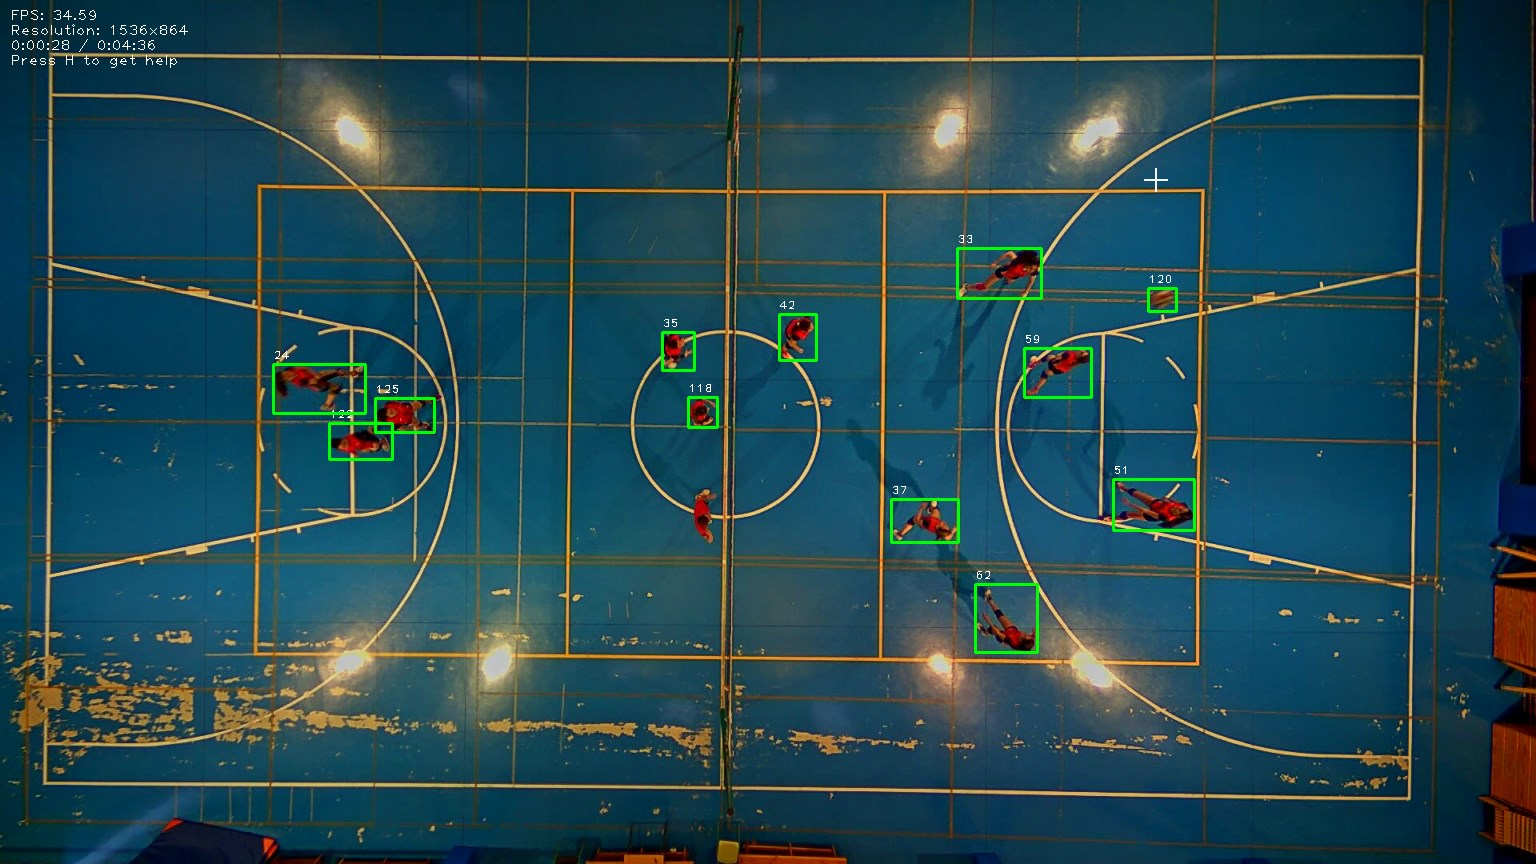
\includegraphics[width=.9\linewidth]{images/noconsistencia}
  \caption { }
  \label{fig:consa}
\end{subfigure}%
\begin{subfigure}{.5\textwidth}
  \centering
  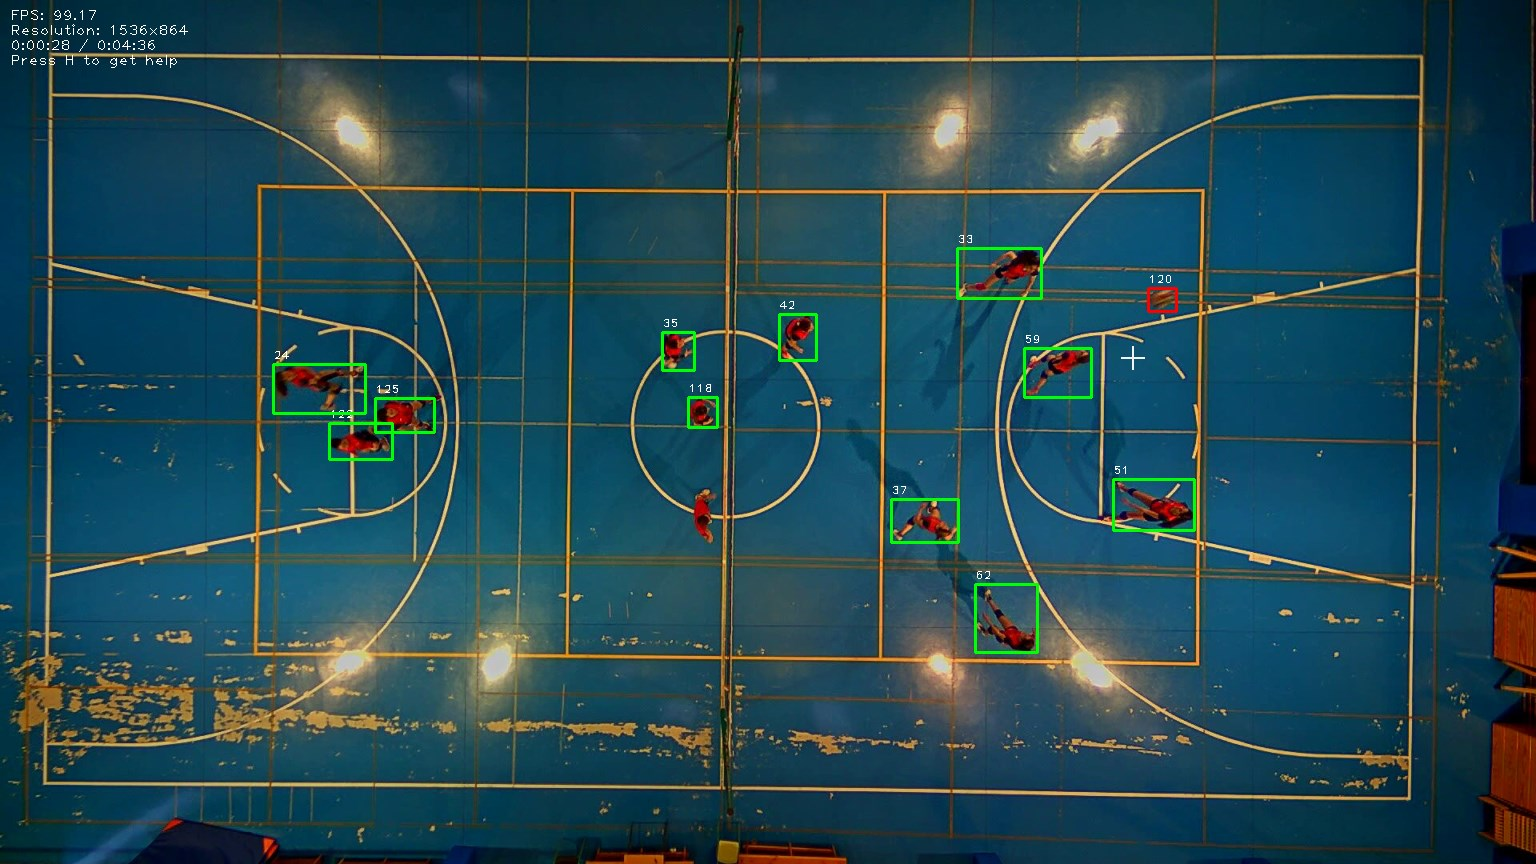
\includegraphics[width=.9\linewidth]{images/consistencia}
  \caption { }
  \label{fig:consb}
\end{subfigure}
\caption{Imagen antes (a) y después (b) de aplicar la técnica de consistencia temporal descrita.}
\label{fig:cons}
\end{figure}

En la figura \ref{fig:cons} podemos ver la diferencia de resultados entre la primera pasada y tras aplicar el algoritmo descrito, la pelota aparece marcada correctamente, mientras que en el frame original en la primera pasada no había ningún contorno marcado como pelota. Además, como en la segunda pasada no necesitamos ejecutar en cada frame la actualización del sustractor de fondo ya que los datos proceden de la pasada anterior, se puede apreciar una mejora significativa de la cifra de FPS.

La tabla \ref{tab:3} presenta los siguientes datos para tres jugadas: número de frames de cada jugada, id del balón, número de frames en que dicha id está marcada como balón antes de aplicar el algoritmo y después, y porcentaje de mejora. Dicho porcentaje de mejora es la diferencia entre el porcentaje de frames con el balón localizado antes de aplicar el algoritmo y después.


\begin{table}
\centering
\begin{tabular}{|c|c|c|c|c|}
\hline
\multirow{2}{2cm}{Número de frames} & \multirow{2}{*}{ball$_{id}$} & \multicolumn{2}{m{4cm}|}{Número de frames en que ball$_{id}$ se marca como balón} & \multirow{2}{2cm}{Porcentaje de mejora} \\ \cline{3-4}
& & \multicolumn{1}{m{2cm}|}{Antes} & \multicolumn{1}{m{2cm}|}{Después} &  \\ \hline
 $185$ & $120$ & $41$ & $145$ & $56.21\%$ \\ \hline
 $135$ & $468$ & $21$ & $75$ & $40\%$ \\ \hline
 $339$ & $754$ & $31$ & $200$ & $49.85\%$ \\ \hline
\end{tabular}
\caption{Análisis de resultados del algoritmo de consistencia temporal implementado. }
\label{tab:3}
\end{table}

Como puede verse, el algoritmo propuesto es bastante efectivo a la hora de localizar el balón en la escena a partir de los datos del sustractor. Hemos sido capaces de encontrar el balón hasta en un $56,20\%$ más de ocasiones que en la salida original. 

Hay que tener en cuenta que el $100\%$ de frames con balón es inalcanzable, ya que hay algunos frames de las jugadas en los que el balón desaparece por solapamiento con una jugadora, por ejemplo. Un coeficiente mejor para determinar el grado de mejora tras aplicar el algoritmo sería el porcentaje de frames en los que se detecta el balón respecto al número total de frames en los que aparece el mismo. Para lograr este último dato necesitamos revisar el vídeo frame a frame de manera manual para crear una verdad de fondo que nos sirva para comparar. Este sería un trabajo demasiado extensivo, por lo que nos conformaremos con las medidas empleadas.


\subsection{Descripción del software final}

El software desarrollado ofrece dos interfaces posibles al usuario final, ambas con la misma funcionalidad. La primera de estas interfaces es la interfaz por consola, la cual se maneja mediante parámetros por línea de comandos, mientras que la segunda es una interfaz gráfica desarrollada usando PyQt.

Dado que, como hemos dicho, ambas ofrecen la misma funcionalidad, el uso de una u otra es simplemente una preferencia personal del usuario en cuestión.

\subsubsection*{Interfaz por consola}
Esta interfaz usa las ventanas estándar de OpenCV (las que pueden verse en la figura \ref{fig:ventanas}) para mostrar el vídeo así como la imagen binarizada que actúa como salida del sustractor de fondo. Para el manejo de parámetros se ha usado el paquete \textit{comargs} que ofrece Python, que permite definir parámetros opcionales, parámetros con número limitado de opciones, etc.

En el caso de esta interfaz, el vídeo se pasa como argumento al ejecutar el programa por línea de comandos. Los parámetros con los que cuenta el programa son:

\begin{itemize}
  \item \textbf{Escala de imagen}: Mediante la opción -s y un factor entre 0 y 1, podemos controlar la escala a la que se procesan y muestran las imágenes del vídeo original. Por ejemplo, un factor de $0,5$ significaría que el vídeo original se reduce a la mitad de su tamaño antes de procesar.
  \item \textbf{Método de sustracción de fondo}: Usando la opción -b se puede seleccionar un método de sustracción de fondo entre todos los expuestos en la sección \ref{sec:subtractors}. En caso de no especificar ninguno, el programa usa el método recomendado, MOG2.
  \item \textbf{Método de tracking}: Podemos seleccionar entre Mean Shift o CAMShift usando la opción -t. De la misma manera que antes, la opción por defecto es Mean Shift.
\end{itemize}

\begin{figure}
\begin{subfigure}{.5\textwidth}
  \centering
  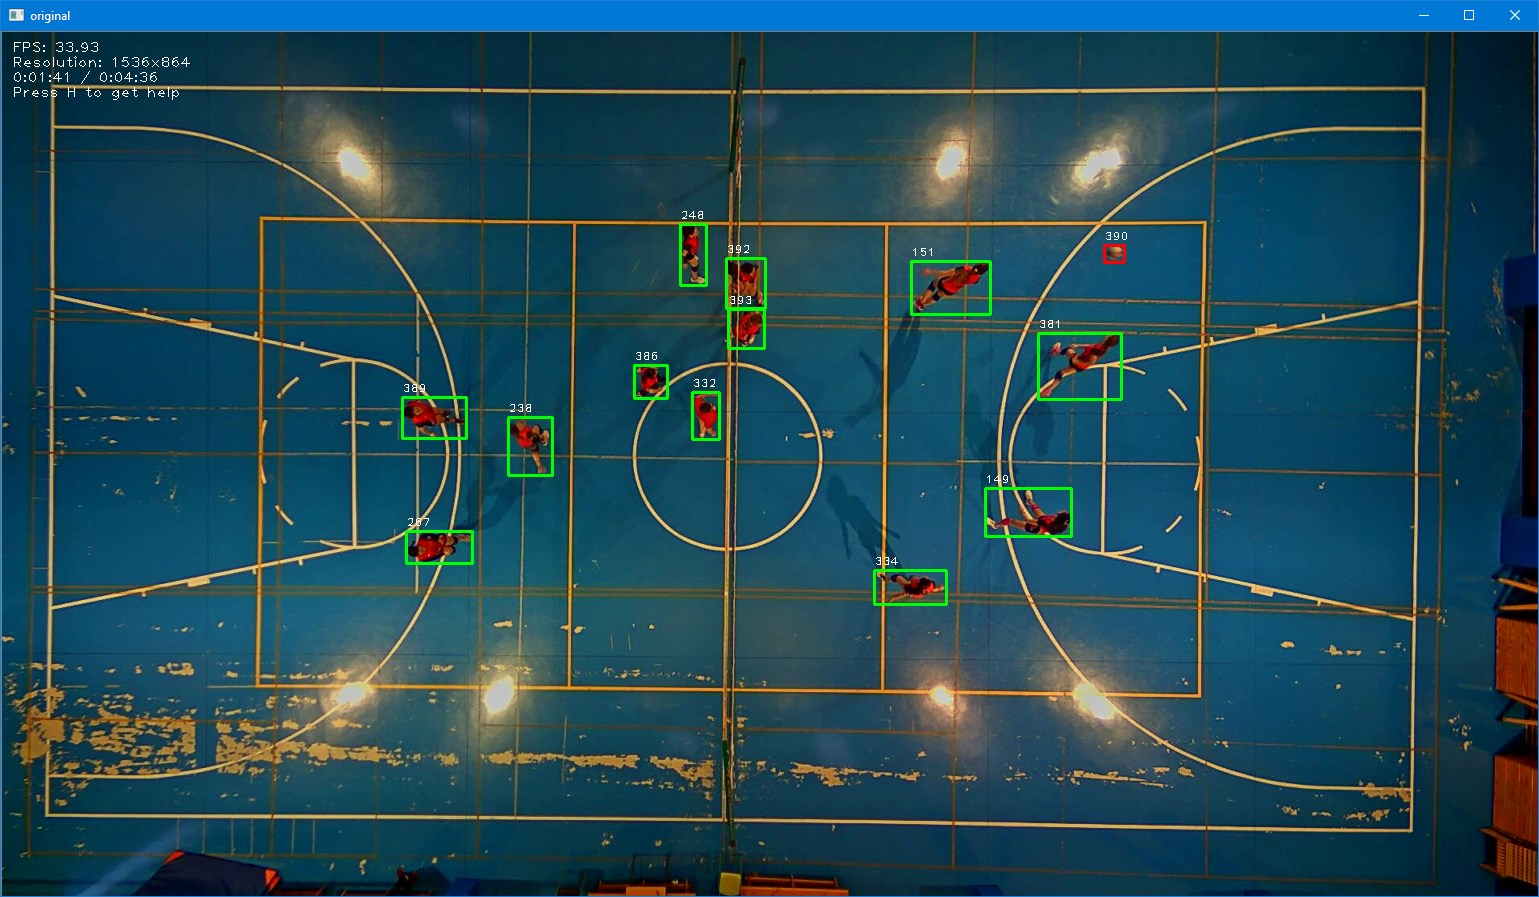
\includegraphics[width=.9\linewidth]{images/original}
  \caption { }
  \label{fig:ventanaoriginal}
\end{subfigure}%
\begin{subfigure}{.5\textwidth}
  \centering
  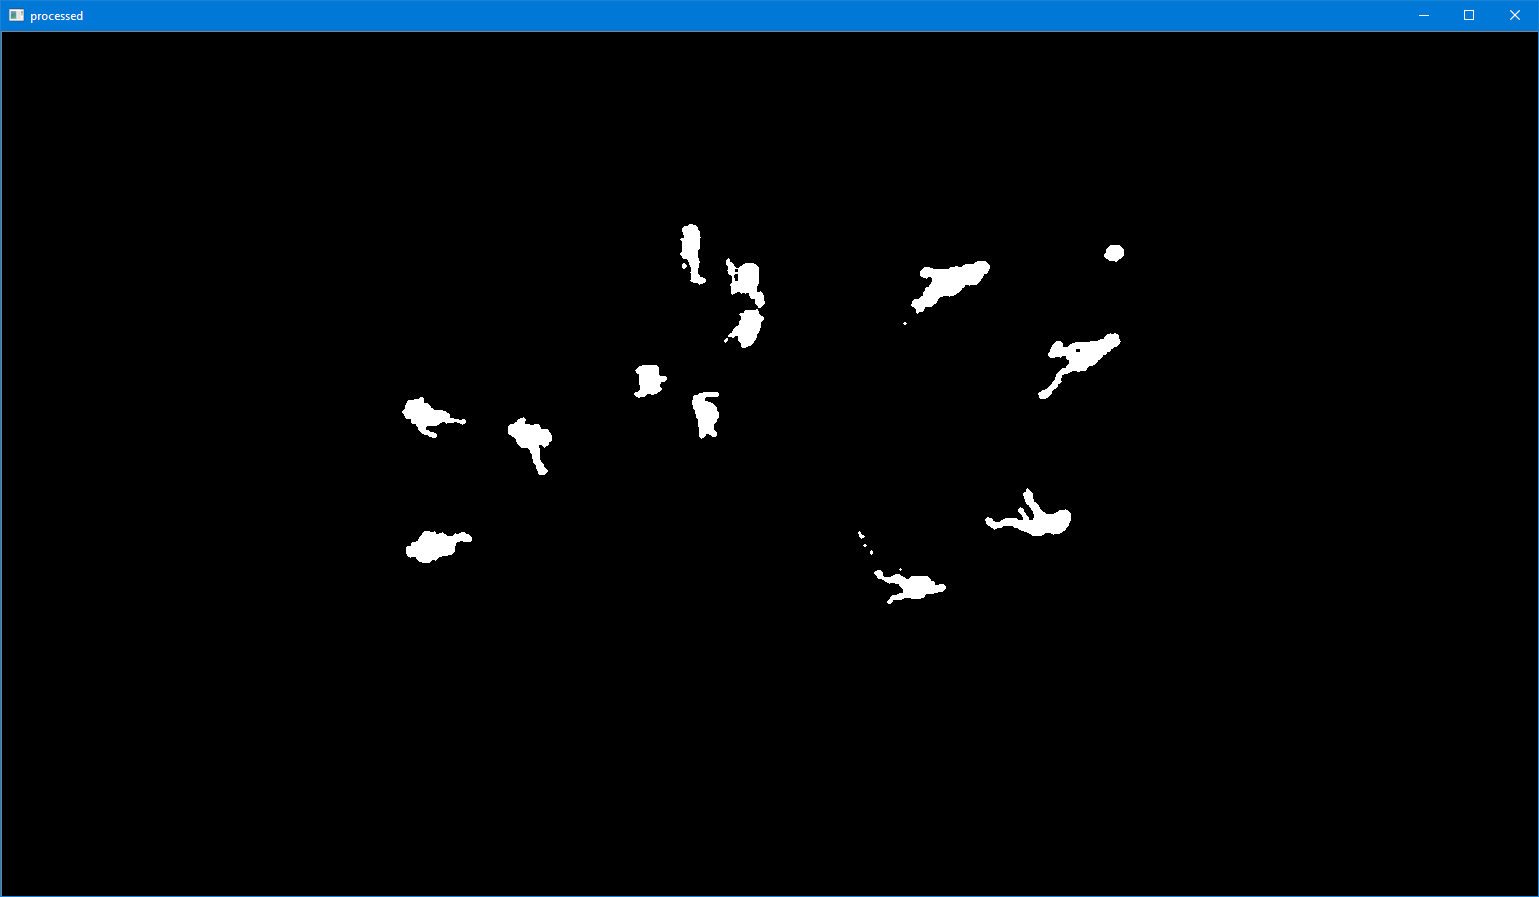
\includegraphics[width=.9\linewidth]{images/processed}
  \caption { }
  \label{fig:ventanaprocessed}
\end{subfigure}
\caption{Ventanas estándar de OpenCV en la interfaz por consola del vídeo (a) y del sustractor de fondo (b).}
\label{fig:ventanas}
\end{figure}

Durante la ejecución del programa puede pausarse el vídeo pulsando la tecla espacio, así como avanzarlo o retrocederlo 5 segundos, usando las teclas K y L respectivamente. Al iniciarse, el programa automáticamente empieza a aplicar el método de sustracción de fondo especificado por parámetro, y pueden verse en la ventana principal recuadros verdes que corresponden con las formas detectadas por el sustractor. Una de estas formas, la marcada en rojo, se corresponde con la pelota.

Dado que para la inicialización de los métodos de tracking se requiere de una ventana inicial desde la que empezar a hacer el seguimiento, en caso de querer usar esta técnica se debe pulsar la tecla T, que hace que se abra una ventana (figura \ref{fig:iniciatracking}) para elegir las regiones iniciales del seguimiento.

Las jugadas, como hemos dicho anteriormente, se detectan de manera manual, por lo que al pulsar la tecla J el programa iniciará el registro de la jugada y lo terminará al volver a pulsar dicha tecla. Al salir del programa se generarán el fichero CSV y un archivo DMP que es el que se usará para la ejecución de la consistencia temporal, pasándolo por parámetro con la opción -l.

\begin{figure}
    \centering
    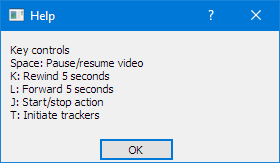
\includegraphics[width=0.4\textwidth]{images/help}
    \caption{Ventana de ayuda de la versión por consola.}
    \label{fig:helpconsola}
\end{figure}

Al pulsar la tecla H, se abre una ventana de ayuda que contiene información sobre todas las funciones de las teclas que se han descrito en esta sección. Dicha ventana es la que aparece en la figura \ref{fig:helpconsola}

\begin{figure}
    \centering
    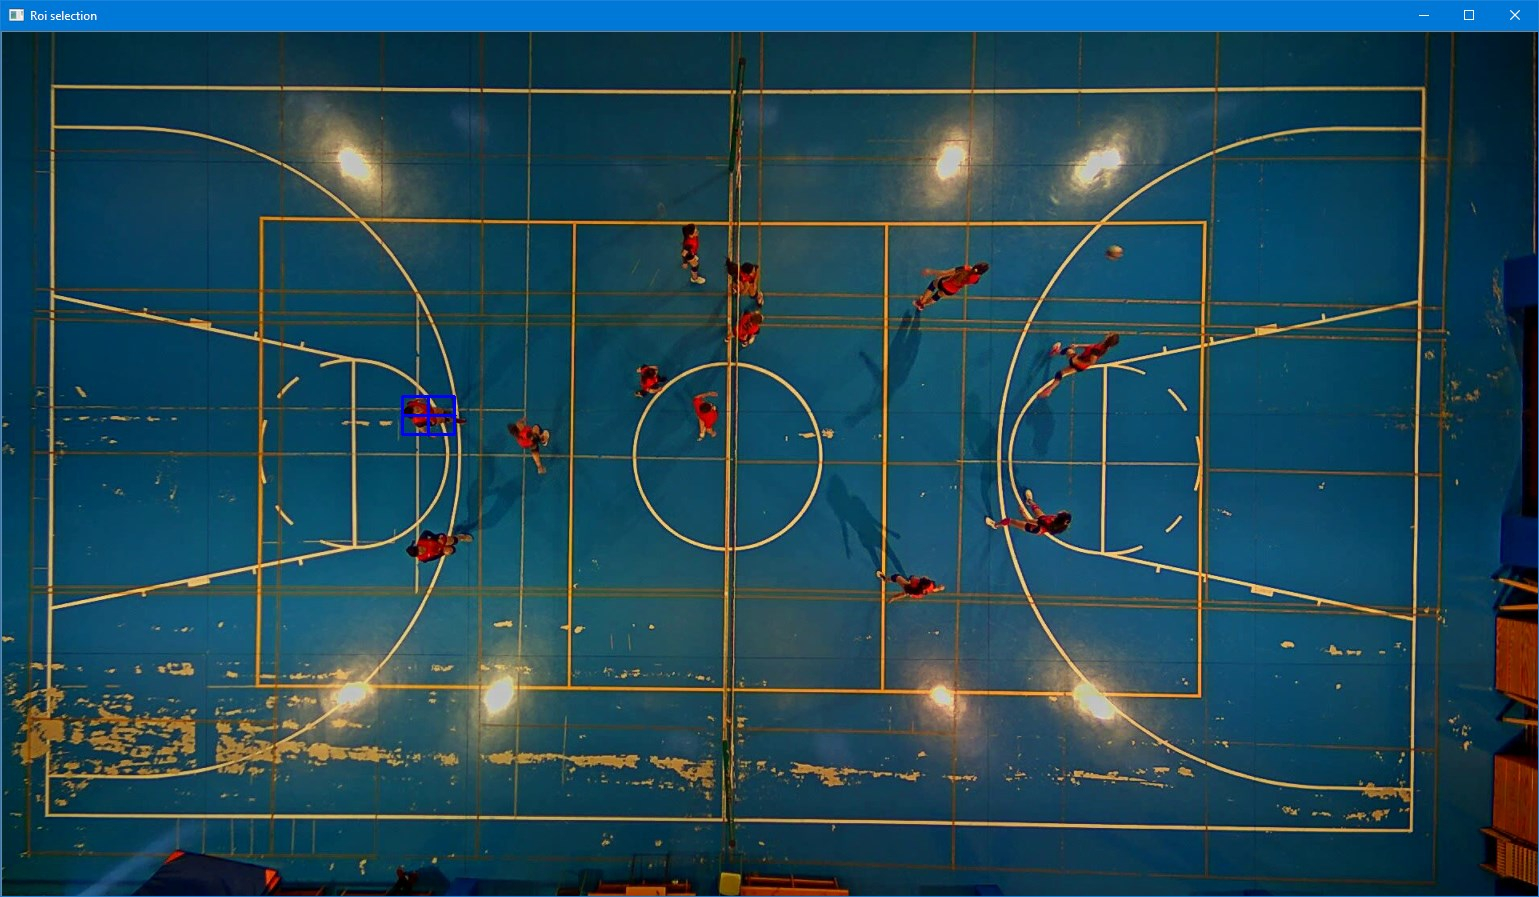
\includegraphics[width=0.8\textwidth]{images/ejemplotracking}
    \caption{Ventana de selección de regiones de interés para tracking.}
    \label{fig:iniciatracking}
\end{figure}

Un ejemplo de ejecución usando esta interfaz seria el siguiente:
\begin{lstlisting}[language=bash]
  ./main.py <Ruta/Al/Video/set_01.avi> -s 0.8 -b MOG2 -l set_01.dmp
\end{lstlisting}

Con este comando, se haría una pasada usando consistencia temporal sobre el vídeo \path{set_01.avi} a escala de imagen $0.8$, usando MOG2 (irrelevante en este caso puesto que la consistencia temporal no llama al sustractor) y con los datos de las jugadas contenidas en \path{set_01.dmp}


\subsubsection*{Interfaz gráfica}
La interfaz gráfica hace empleo de la biblioteca gráfica PyQt. Esta parte de la aplicación cuenta con la misma funcionalidad que la anterior, pero puede resultarle más sencilla de manejar al usuario medio.

En este caso no es necesario especificar parámetros por consola puesto que todo se controla desde la interfaz desarrollada. Las distintas posibilidades que ofrece son:

\begin{figure}
    \centering
    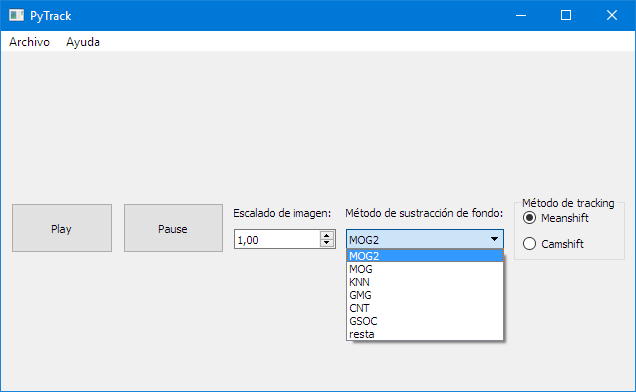
\includegraphics[width=0.4\textwidth]{images/combobox}
    \caption{Desplegable con los métodos de sustracción de fondo disponibles.}
    \label{fig:combobox}
\end{figure}

\begin{itemize}
  \item \textbf{Seleccionar el vídeo} mediante el menú Archivo, que muestra una ventana del sistema para buscar la ruta del vídeo.
  \item \textbf{Controlar la escala} mediante un cuadro numérico que va de 0 a 1.
  \item \textbf{Seleccionar el método de sustractor} con un desplegable (figura \ref{fig:combobox}). Los métodos posibles son los expuestos en la sección \ref{sec:subtractors}.
  \item \textbf{Elegir el método de seguimiento} ente Mean Shift y CAMShift.
\end{itemize}

De la misma manera que en la versión por consola, el software admite el uso de teclas para ciertas funciones. Además de los atajos, que omitiremos por su poco interés, se permite seleccionar las ventanas iniciales del seguimiento usando la tecla T, que abrirá una ventana en la que seleccionar las regiones de interés.

\begin{figure}
    \centering
    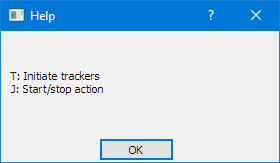
\includegraphics[width=0.4\textwidth]{images/help2}
    \caption{Ventana de ayuda de la interfaz gráfica.}
    \label{fig:help}
\end{figure}

También podemos capturar jugadas del mismo modo que en la otra versión: pulsando una tecla al principio y al final de cada jugada. Nuevamente, tenemos una ventana de ayuda (figura \ref{fig:help}) a nuestra disposición que nos indica qué teclas hacen cada función.

\begin{figure}
\begin{subfigure}{.5\textwidth}
  \centering
  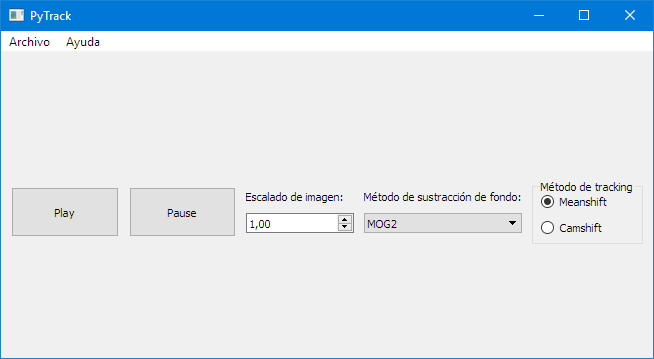
\includegraphics[width=.9\linewidth]{images/ventanagrafica}
  \caption { }
  \label{fig:graficaA}
\end{subfigure}%
\begin{subfigure}{.5\textwidth}
  \centering
  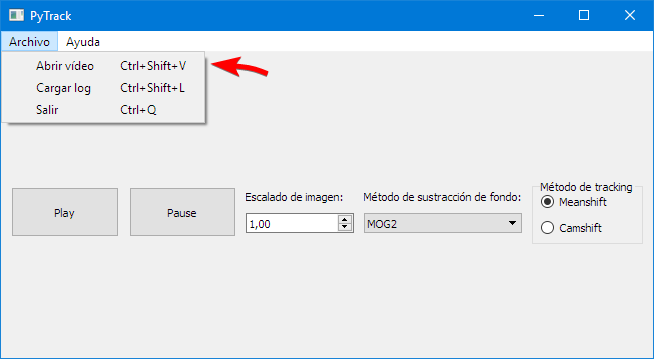
\includegraphics[width=.9\linewidth]{images/ventanacargar}
  \caption { }
  \label{fig:graficaB}
\end{subfigure}
\caption{Pantalla de inicio de la interfaz gráfica (a) y ventana con el menú para cargar vídeo (b).}
\label{fig:grafica}
\end{figure}

En la figura \ref{fig:grafica} puede verse la ventana principal de la aplicación, así como los menús que nos permiten cargar vídeos y logs. Una vez cargado un vídeo, al pulsar el botón Play comenzará a ejecutarse el programa con normalidad y aparecerá un slider que permite controlar el momento del vídeo al que se quiere ir, en caso de querer saltar.

Al iniciar la reproducción del vídeo, tanto usando consistencia temporal como sin usarla, la ventana se ve como en la figura \ref{fig:ventanaconvideo}. Tenemos la posibilidad de ver la salida del sustractor de fondo, desmarcando el checkbox \texttt{Video output}.

\begin{figure}
    \centering
    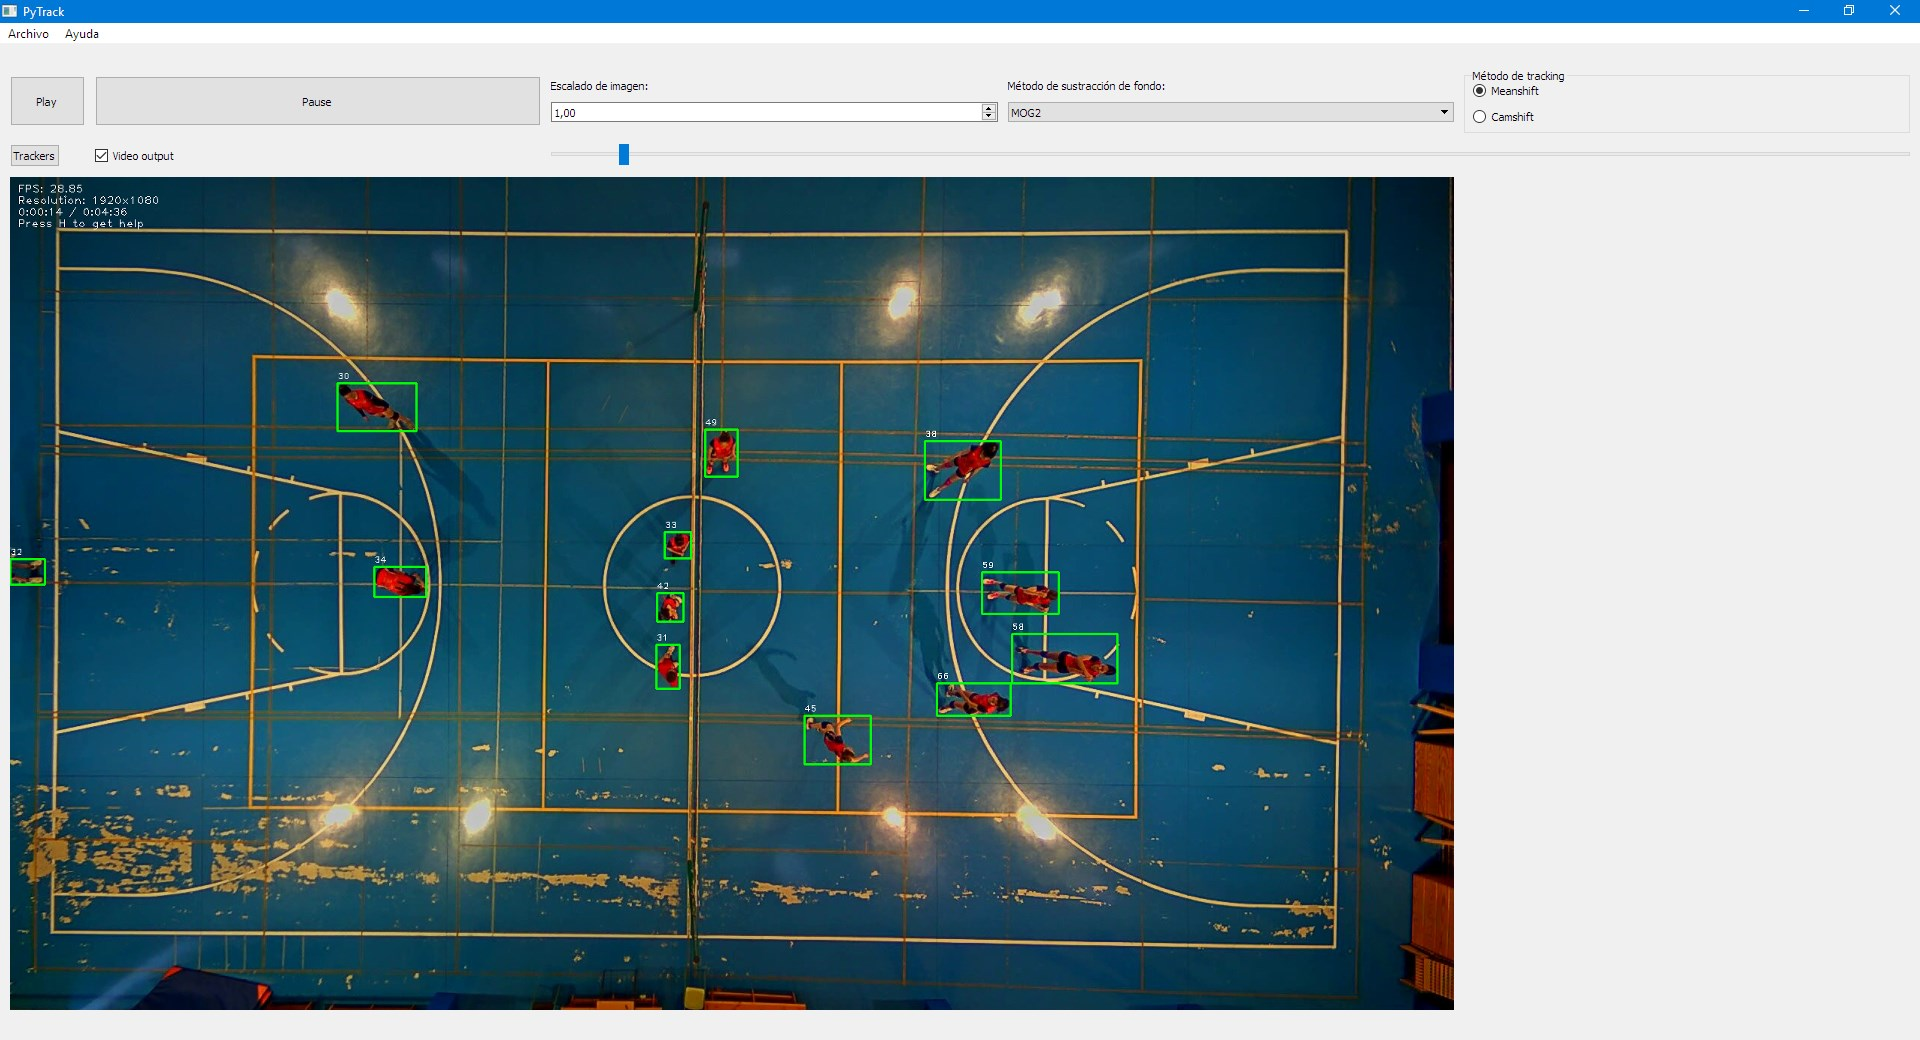
\includegraphics[width=0.75\textwidth]{images/grafica}
    \caption{Ventana de la interfaz gráfica mientras se procesa un vídeo.}
    \label{fig:ventanaconvideo}
\end{figure}

\newpage